\documentclass[UTF8,lettersize,journal]{IEEEtran}
\usepackage{ctex}
\usepackage{amsmath,amsfonts}
\usepackage{algpseudocode}
\usepackage{algorithm}
\usepackage{array}
\usepackage{amssymb}
\usepackage{amsthm}
\usepackage{enumitem}
\usepackage[caption=false,font=small,labelfont=rm,textfont=rm]{subfig}
\usepackage{textcomp}
\usepackage{stfloats}
\usepackage{url}
\usepackage{verbatim}
\usepackage{graphicx}
\usepackage{cite}
\usepackage{bm}
\usepackage[acronym]{glossaries}
\usepackage{mathrsfs}
\usepackage{indentfirst}
\usepackage{multirow}
\usepackage{float}
\usepackage{color}
\usepackage{subfig}
\usepackage{subcaption}
\usepackage{booktabs}
\usepackage[switch]{lineno}
\algrenewcommand{\algorithmicrequire}{\textbf{输入:}}
\algrenewcommand{\algorithmicensure}{\textbf{输出:}}
\hyphenation{op-tical net-works semi-conduc-tor IEEE-Xplore}

\begin{document}

\title{基于扩散增强可信多模态大语言模型的抗幻觉滚动机械故障诊断}
%LLM-Augmented Causal Invariant Learning: \ A Two-Stage Fine-Tuning Approach for Single-Source Open-Set Vehicle Fault Diagnosis
%LLM-Augmented Causal Invariant Learning: \ A Cycling Fine-Tuning Approach for Single-Source Open-Set Vehicle Fault Diagnosis

% The paper headers
\markboth{J. of \LaTeX\ C. F.}%
{Shell \MakeLowercase{\textit{et al.}}: A Sample Article Using IEEEtran.cls for IEEE Journals}

% Remember, if you use this you must call \IEEEpubidadjcol in the second
% column for its text to clear the IEEEpubid mark.

\maketitle

\begin{abstract}
大语言模型(LLMs)在机械系统故障诊断中表现出优异性能，但其响应中潜在的事实性错误会削弱LLMs的可信度。
这些事实性错误通常被称为幻觉，阻碍了LLMs在安全关键环境中的部署。
由于其自回归生成机制，当受到嵌入在权重中的统计偏差或领域无关提示触发时，LLMs可能会生成流畅但虚构的响应。
此外，大量形式正确但语义空洞的响应掩盖了局部幻觉的迹象。
为解决这些问题，我们提出了一种扩散增强可信多模态大语言模型(DA-TMLLM)。
首先，我们设计了一个ControlNet引导的跨数据集条件扩散模型(CGCDM)，通过注入可控语义引导和合成多样化样本来缓解统计偏差。
其次，我们设计了一个TMLLM，通过点二列相关分析和显著性检验来定位关键token，并设计关键token驱动的不确定性重加权策略，以增强幻觉检测性能。
第三，我们设计了一个抗幻觉方案用于幻觉缓解和检测，将CGCDM和TMLLM整合到一个统一的流程中，并详细说明了拒绝领域无关提示的过程。
在十一个数据集上获得的评估结果表明，我们提出的DA-TMLLM在八个指标上始终优于十一个对比模型。
\end{abstract}
%全文有关数据集、对比算法的数量、对比指标的数量最后需要核对，包括摘要、贡献最后一条、实验部分第一段和结论。
\begin{IEEEkeywords}
可信多模态大语言模型，抗幻觉，扩散增强，ControlNet，关键token定位，不确定性重加权策略。


\end{IEEEkeywords}

\section{引言}
\IEEEPARstart{大}{型}机械设备，从高速列车到海上钻井平台，对现代工业基础设施至关重要。
滚动轴承作为机械的关键部件，承担着减少摩擦和支撑载荷等多种重要功能，通常在恶劣环境下运行\cite{PU, JUST}。
因此，对运行数据进行持续监测并快速诊断故障特征对于确保安全至关重要。
得益于信号采集技术和人工智能的发展，数据驱动的诊断方法已成为主流方法论，能够从历史数据中自动得出诊断结果\cite{10577994, HIT}。

近年来，大语言模型(LLMs)因其优越性能已逐步取代传统深度学习模型(CDLMs)用于故障诊断\cite{Peng_Liu_Du_Gao_Wang_2025}。
这些模型能够在多种工况下提供准确的诊断结果和维护建议。
尽管取得了这些进展，但最关键的一种失效模式，即``幻觉''，仍然是一个突出问题。
幻觉指的是LLM生成的长文本回答中包含事实性错误的情况，例如错误的诊断结果或不恰当的维护建议\cite{li-etal-2023-halueval, azaria-mitchell-2023-internal}。
在实际部署中，真实标签通常不可用，因此难以确定LLM生成的响应是否包含事实性错误。
此类错误信息可能造成重大经济损失甚至危及人身安全。
然而，在消除LLM生成回答中的事实性错误和检测幻觉方面仍存在若干挑战。

\textbf{统计偏差诱导的幻觉}。
工业滚动轴承在其大部分使用寿命中通常保持健康状态，这使得轴承数据集本质上呈现不平衡的长尾分布。
不平衡的训练集会使学习到的决策边界产生偏差，并将统计偏差引入LLMs，导致它们倾向于多数类。
因此，大量的正常类别和任何相对频繁出现的故障模式主导了梯度更新，成为偏差的主要来源。
在推理过程中，如果输入样本属于少数(尾部)类别，模型仍然倾向于预测更常见的类别，这可能导致对罕见但安全关键故障的漏报。


\textbf{不期望输入诱导的幻觉}。
部署后，LLMs可能会遇到不期望的输入，例如来自以前未见过的旋转机械类型的传感器信号或其他领域无关的信号源。
当面对此类输入时，LLMs经常通过产生流畅但虚构的回答来产生幻觉，而不是拒绝查询。
这是因为当前的LLMs缺乏对其认知极限的明确意识，不知道何时沉默才是适当的回应。
此外，如果不期望的输入与训练数据表现出强烈的语义重叠(例如，来自新型轴承但与已知数据相似的信号)，LLM可能变得过于自信并为此输入分配高后验概率。


\textbf{序列级幻觉的隐蔽性}。
对于回答序列中的每个token，其后验概率主要受模型内部先验、语料级词频和局部句法模式的影响，而不是该token与训练数据的匹配程度。
因此，当检测器仅基于token级后验进行判断时，幻觉可能会逃脱检测。
此外，在评估整个回答序列时，我们发现许多形式正确但语义空洞的短语，例如``\textit{从提供的列表中最合适的轴承状态类型是}''。
这种语言冗余的存在往往会稀释幻觉内容。
因此，即使回答序列中存在幻觉，幻觉量化指标仍可能给出正常值。

为解决这些问题，我们提出了一种扩散增强可信多模态大语言模型(DA-TMLLM)。
首先，我们设计了一个ControlNet引导的跨数据集条件扩散模型来缓解统计偏差诱导的幻觉。
其次，我们通过在多个轴承数据集上的文本-信号对微调预训练LLM，开发了一个TMLLM。
在开发的TMLLM基础上，我们识别关键token并设计关键token驱动的不确定性重加权策略来有效检测序列级幻觉。
第三，我们设计了一个抗幻觉方案用于幻觉缓解和检测，将CGCDM和TMLLM整合到一个统一的流程中，并详细说明了拒绝不期望输入的过程。 % explicitly addresses how to reject undesired inputs.
DA-TMLLM的贡献如下：
\begin{enumerate}[] 
	\item[1)] 我们设计了一个ControlNet引导的跨数据集条件扩散模型。
	通过注入可控语义引导，该模型在保持语义一致性的同时增强了合成样本的多样性。
	\item[2)] 我们通过定位关键token并设计关键token驱动的不确定性重加权策略，设计了一个可信多模态大语言模型，显著提高了LLM的幻觉检测性能。
	\item[3)] 我们设计了一个抗幻觉方案，将CGCDM和TMLLM整合到一个统一的流程中，并结合不期望输入拒绝方法。该方案在缓解LLM幻觉的同时进一步提高了检测性能。
	% We design a hallucination-resilient scheme. By integrating CGCDM and TMLLM into a unified pipeline and developing an undesired input rejection method, the design scheme further enhances detection performance while alleviating LLM hallucinations.
	\item[4)] 在十一个数据集上获得的评估结果表明，DA-TMLLM在八个指标上始终优于十一个对比模型。
\end{enumerate}

本文结构如下。
第二节回顾了与故障诊断和幻觉检测相关的LLMs和CDLMs。
第三节详细介绍了提出的用于抗幻觉故障诊断的DA-TMLLM。
第四节评估了DA-TMLLM的性能并展示了实验结果。
第五节对本文进行总结。

\section{相关工作}
% In this section, we review the related methods including CDLMs and LLMs for mitigating statistical bias, CDLMs and LLMs for rejecting undesired data, and LLMs for detecting sequence-level hallucinations.
在本节中，我们回顾了相关方法，包括(1)用于缓解统计偏差的CDLMs和LLMs，(2)用于拒绝不期望输入的CDLMs和LLMs，以及(3)用于检测序列级幻觉的LLMs。

\subsection{用于缓解统计偏差的CDLMs和LLMs}
在\cite{Peng_Liu_Du_Gao_Wang_2025}中，H. Peng \emph{et al.}设计了一个跨数据集诊断LLM，称为BearLLM。
在\cite{VGCDM}中，X. Liu \emph{et al.}将脉冲电压嵌入引入扩散过程以实现可控振动合成。
在\cite{DCGAN}中，K. Zhou \emph{et al.}开发了一个平衡生成器-判别器架构用于诊断齿轮缺陷，称为DCGAN。
在\cite{WOS:000688310200005}中，T. Han \emph{et al.}提出了一个混合网络，结合类别约束和对抗域正则化来捕获可迁移特征。
在\cite{10478558}中，M. Vu \emph{et al.}提出了一个双分支诊断框架，以提高稀疏标签场景下的故障分类准确率。
在\cite{QSCGAN}中，W. Wan \emph{et al.}在生成器-判别器架构中嵌入自注意力和谱归一化来增强火箭轴承数据，称为QSCGAN。
在\cite{VQVAE}中，Q. Zheng \emph{et al.}结合退化阶段划分和向量量化增强来丰富退化特征，称为VQVAE。



\subsection{用于拒绝不期望输入的CDLMs和LLMs}
%MDCC=DSRC+马氏距离
%WDSN=DANN+马氏距离
在\cite{ZHAO2022108672}中，C. Zhao \emph{et al.}采用三元组损失和边界自适应方法来学习紧凑特征和最优类别边界。
在\cite{10262196}中，Z. Zhu \emph{et al.}开发了一个对抗训练的开放集分类器来识别未知类别和域外样本。
在\cite{10214410}中，J. Long \emph{et al.}通过将元学习块与马氏距离相结合，开发了一个域泛化未见故障诊断方法，称为MLMM。
在\cite{ZHANG2023109518}中，X. Zhang \emph{et al.}引入了一种域自适应方法，解耦私有和共享特征来诊断未见故障，称为WDSN。
在\cite{10382502}中，B. Lu \emph{et al.}设计了一个基于对比嵌入的诊断策略，联合保留域特定和域不变特征，称为MDCC。
在\cite{20242516270368}中，B. Liu \emph{et al.}对LLaMA系列LLMs进行不期望输入检测的基准测试，并使用各向同性嵌入设计了一个基于余弦距离的检测器，称为LLM-OOD。


\subsection{用于检测序列级幻觉的LLMs}
%请检查LLM-check中具体用到的特征，确保与实验一致。
%请检查\cite{azaria-mitchell-2023-internal}是否是秒杀级对比算法 <- 这篇论文没开源
%请检查这篇论文Detecting Hallucinations in Large Language Model Generation: A Token Probability Approach，参考文献中有好多利用中间层信息进行幻觉检测的文献。
%请检查Unsupervised Real-Time Hallucination Detection based on the Internal States of Large Language Models是否是秒杀级对比算法 <- 使用LLM-Check-HiddenScore实现
在\cite{20251218102787}中，G. Sriramanan \emph{et al.}设计了一个计算高效的检测器，利用模型的内部注意力图，称为LLM-Check。
在\cite{20243917091282}中，J. Duan \emph{et al.}通过重加权token级和序列级相关性，开发了一种幻觉量化方法。
在\cite{20240715556058}中，T. Zhang \emph{et al.}引入了一个无需检索的检测器，通过token级不确定性来量化幻觉。
在\cite{selfcheckgpt}中，P. Manakul \emph{et al.}提出了SelfCheckGPT，通过采样多个黑盒LLM响应并测量它们的一致性来评估幻觉。
% In \cite{azaria-mitchell-2023-internal}, A. Azaria \emph{et al.} design a hallucination classifier using LLM hidden activations.
在\cite{su-etal-2024-unsupervised}中，W. Su \emph{et al.}提出了一个使用LLMs内部状态的实时无标注幻觉检测框架，称为MIND。
在\cite{10.1007/978-3-031-86623-4_13}中，E. Quevedo \emph{et al.}提出了一个有监督方法，利用在资源高效的数值特征上训练的辅助检测器，称为SHalluDetect。
% In \cite{20242516270368}, B. Liu \emph{et al.} highlight the isotropic nature of LLMs and design a cosine distance-based hallucination detector, termed LLM-OOD.
在\cite{li-etal-2023-halueval}中，J. Li \emph{et al.}通过采样-过滤和标注开发了一个用于幻觉分析的基准。

然而，在提高诊断LLMs性能方面仍存在若干开放问题。
首先，现有模型忽视了由数据集间差异和类别不平衡共同造成的复合统计偏差，经常将域特定特征误认为随机噪声。
简单的基于扰动的增强通过生成强相关样本来进一步加剧这一问题，这些样本无法有效丰富少数类。
其次，CDLMs和LLMs倾向于低估与和训练数据共享高级语义的不期望输入相关的预测不确定性，从而降低诊断准确率。
第三，由于生成文本中的语义冗余和模型的过度自信，现有检测器经常无法识别幻觉内容。
为解决这些问题，我们提出了DA-TMLLM，通过有效增强训练数据和准确量化生成回答的不确定性来检测和缓解LLM幻觉。


\section{方法}
%\mathcal{} 表示函数
%\mathrm{} 多字符下标，标量下表都用直立体
%有关概率的q和P符号需要检查

\begin{figure*}[!t]
	\centering
	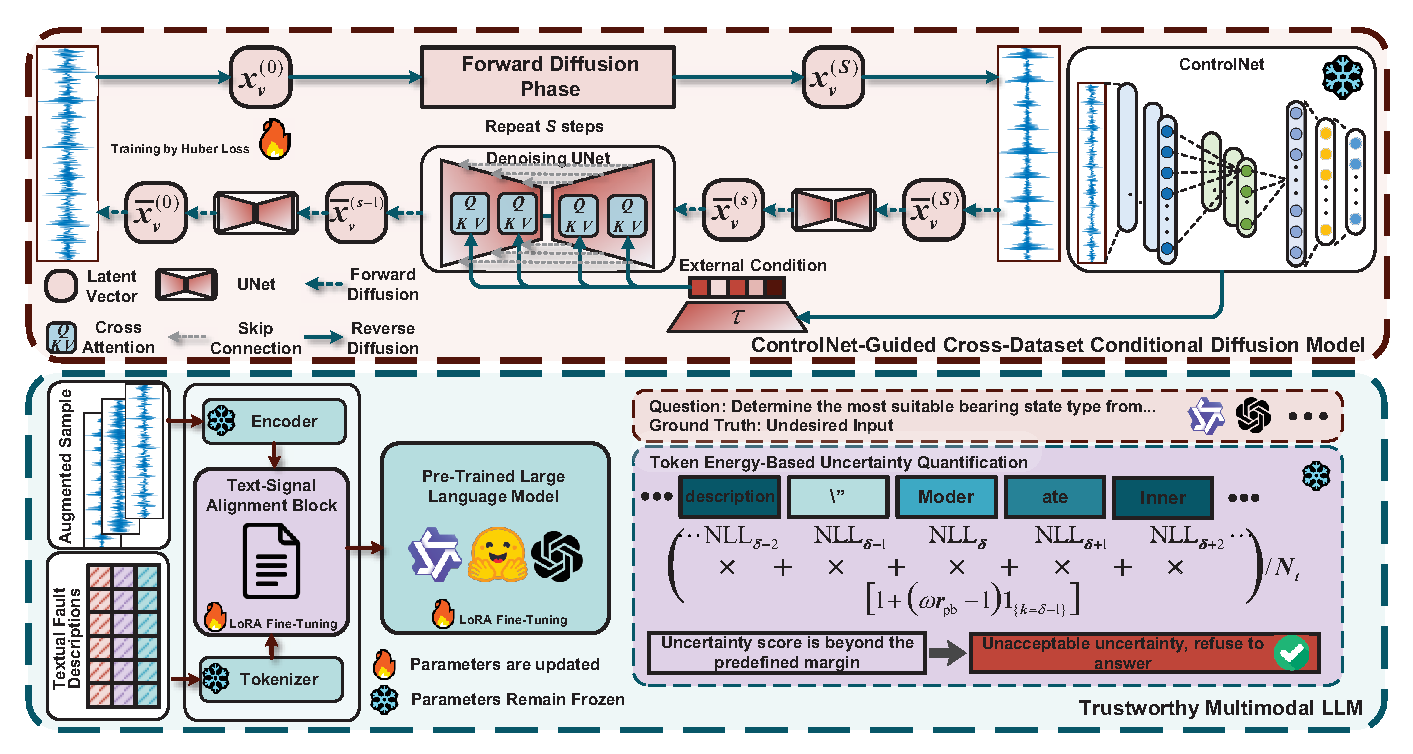
\includegraphics[width=7in]{figures/whole_framework.eps}
	\caption{所提出的DA-TMLLM的整体框架。(a) CGCDM(可控引导条件扩散模型)注入语义引导以缓解统计偏差诱导的幻觉。(b) TMLLM(可信多模态大语言模型)通过定位关键token并开发关键token驱动的不确定性重加权策略来检测序列级幻觉。(c) 基于DA-TMLLM设计了抗幻觉方案，开发了训练和推理流程，并详细说明了拒绝不期望输入的过程(详见第\ref{sec:scheme}节)。}
	\label{fig_framework}
\end{figure*}

所提出的DA-TMLLM的整体框架如图\ref{fig_framework}所示。
首先，我们介绍设计的ControlNet引导跨数据集条件扩散模型(CGCDM)来缓解统计偏差诱导的幻觉。
其次，我们介绍可信多模态大语言模型，包括微调、关键token定位和关键token驱动不确定性重加权策略的详细信息。
第三，我们介绍基于DA-TMLLM的抗幻觉方案。

\subsection{ControlNet引导的跨数据集条件扩散模型}
为缓解数据集间差异，我们提出了一种跨数据集标准化方法，包括固定时长分割、长度对齐和尺度归一化。
然后，我们开发了条件扩散模型(CDM)的架构来合成振动信号。
最后，我们设计了一个ControlNet在反向扩散阶段注入可控语义引导。
\subsubsection{数据预处理的跨数据集标准化方法}
由于不同轴承数据集的传感器采样率、采集条件和轴承类型差异很大，采集的信号在特征故障频率和幅度上存在差异。
当这些异构信号直接输入扩散模型时，模型倾向于将数据集间差异视为随机噪声，阻碍其学习有效的联合分布。
为解决这一问题，我们提出了一种跨数据集标准化方法。

在传统的数据预处理方法中，原始时域信号通常被分割成包含相同数据点数的固定长度样本。
由于振动信号以不同的采样率采集，固定长度分割方法会改变特征故障频率，从而扩大数据集间差异。
为缓解这一问题，我们引入了固定时长分割方法，第$m$个片段表示为
\begin{equation}
\bm{x}_o = \bigl\{\, \bm{x}_r[i] \bigm| i = m\nu,\, m\nu+1,\, \dots,\; (m+1)\nu - 1 \bigr\},
\end{equation}
其中$\nu$是数据集特定的采样率，$\bm{x}_r$是原始信号。
经过固定时长分割后，来自不同数据集的片段需要进一步在长度和幅度上对齐以作为合适的网络输入。
这通过依次应用离散傅里叶余弦变换和尺度归一化来实现，分别表示为$\operatorname{DFCT}(\cdot)$和$\operatorname{SNorm}(\cdot)$。
$\operatorname{DFCT}(\cdot)$将时域片段转换为其频谱，之后仅保留前$L_{f}$个频谱bin，其中$L_{f}$是预定义长度。为适应采样率的变化，包含少于$L_{f}$个bin的频谱进行零填充，而包含更多的则被截断。
然后，所得频谱的幅度通过$\operatorname{SNorm}(\cdot)$映射到区间$\left[-1,1\right]$。
% The successive preprocessing process is expressed as
该预处理过程表示为
\begin{equation}
	\label{eq:dcn}
	\bm{x}_v =
	\begin{cases}
		\operatorname{SNorm}\bigl(\operatorname{DFCT}(\bm{x}_o)[0:L_{f}]\bigr),      & \ell \ge L_{f},\\[4pt]
		\operatorname{SNorm}\bigl(\operatorname{Concat}(\operatorname{DFCT}(\bm{x}_o),\bm{0}_{\,L_{f}-\ell})\bigr), & \ell < L_{f},
	\end{cases}
\end{equation}
其中$\ell$是实际频谱bin数，$\operatorname{SNorm}(\cdot)$表示为
\begin{equation}
	\label{eq:scalenorm}
	\operatorname{SNorm}(\bm{x})=g\,\frac{\bm{x}}{\lVert \bm{x}\rVert_{2}},
\end{equation}
其中$g=\rho\sqrt{L_{f}}$，$\rho$是预定义的缩放因子。


\subsubsection{ControlNet引导的条件扩散}
我们采用基于扩散的增强模型，同时促进训练稳定性和样本多样性，它由前向扩散阶段和反向扩散阶段组成。
为增强生成过程中的语义一致性，我们设计了一个ControlNet，在每个反向扩散步骤将高级语义特征注入潜在特征。

在前向扩散过程中，预处理后的$\bm{x}_v$通过长度为$S$的马尔可夫链逐步添加噪声，其中各向同性的高斯噪声在每一步$s \in \{1,\dots ,S\}$递增添加。
第$s$步的加噪过程表示为
\begin{equation}
q(\bm{x}_v^{(s)} \mid \bm{x}_v^{(s-1)}) = \mathcal{N}\!\bigl(\sqrt{\alpha^{(s)}}\,\bm{x}_v^{(s-1)},\, (1-\alpha^{(s)})\bm{I}\bigr),
\end{equation}
其中$\bm{I}$是单位矩阵，$\alpha^{(s)}$是噪声缩放因子，$\alpha^{(s)} = 1 - \beta^{(s)}$，$\beta^{(s)}$由预定义的方差调度$\zeta$指定。
经过$S$步后，$\bm{x}_v^{(S)}$接近纯高斯样本分布。
使用闭式累积，整个前向扩散过程可表示为
\begin{equation}
q(\bm{x}_v^{(S)} \mid \bm{x}_v^{(0)}) = \mathcal{N}\!\bigl(\sqrt{\hat{\alpha}^{(S)}}\,\bm{x}_v^{(0)},\,(1-\hat{\alpha}^{(S)})\bm{I}\bigr),
\end{equation}
其中$\hat{\alpha}^{(S)} = \prod_{s=1}^{S} {\alpha}^{(s)}$。
$\bm{x}_v^{(S)}$作为后续反向扩散阶段的输入。

在反向扩散阶段，初始潜在变量
$\bm{x}_v^{(S)} \sim \mathcal{N}(0,\bm{I})$由步感知去噪器$\epsilon_{\bm{\theta}_\mathrm{d}}(\cdot)$迭代细化。
在每个扩散步骤$s$，基于UNet的噪声预测网络接收三元组
$(\bar{\bm{x}}_v^{(s)},\,s,\,\bm{c})$，估计添加的高斯扰动，并计算后验均值
\begin{equation}
	\mu_{{\theta}_\mathrm{d}} \bigl(\bar{\bm{x}}_v^{(s)},\,s,\,\bm{c}\bigr)
	= \frac{\bar{\bm{x}}_v^{(s)} - \sigma^{(s)} \epsilon_{{\theta}_\mathrm{d}} \bigl(\bar{\bm{x}}_v^{(s)}, s, \bm{c}\bigr)}
	{\sqrt{\bar{\alpha}^{(s)}}},
\end{equation}
其中$\bar{\alpha}^{(s)} = 1-\bar{\beta}^{(s)}$，$\sigma^{(s)} = \sqrt{1-\bar{\alpha}^{(s)}}$，$\bm{c}$是外部条件向量。
$\bm{c}$通过向噪声预测网络注入辅助信息，在整个反向扩散阶段提供可控引导。
然后从$\mathcal{N} \bigl(
\mu_{{\theta}_\mathrm{d}} \bigl(\bar{\bm{x}}_v^{(s)},\,s,\,\bm{c}\bigr), \bigl(\sigma^{(s)}\bigr)^{2}\bm{I}\bigr)$采样新的潜在变量$\bar{\bm{x}}_v^{(s-1)}$。
对所有$s = S,\ldots,1$重复此随机重建逐步抑制注入的噪声，最终输出$\bar{\bm{x}}_v^{(0)}$收敛到学习的数据分布，从而产生真正的合成样本。

为向反向扩散阶段注入可控语义引导，我们设计了一个ControlNet，将辅助知识嵌入为低维外部条件向量$\bm{c}$。
具体来说，设计的ControlNet首先在标注的振动信号上进行预训练，并优化以将每个原始信号映射到类别判别潜在表示。
为构建对数据集间差异具有鲁棒性的外部条件向量，我们采用三元组输入$\bm{H}_{v} = \bigl[\bm{x}_{v},\;\tilde{\bm{x}}_{v},\;\bm{x}_{vr}\bigr]\in\mathbb{R}^{3 \times L_{f}}$，其中$\bm{x}_{v}$是生成的查询样本，$\tilde{\bm{x}}_{v}$是无故障信号样本，$\bm{x}_{vr}=\bm{x}_{v}-\tilde{\bm{x}}_{v}$是放大故障相关偏差的残差样本。
如图\ref{fig_controlnet}所示，ControlNet的编码器由三个大核卷积通道组成，随后是三个跨通道注意力块(CCAB)，用于跨尺度融合特征。
然后，编码器的输出被送入一个两层全连接分类器，ControlNet通过分类交叉熵损失进行训练。
在扩散模型训练期间，ControlNet的编码器和分类器权重，表示为$\bm{\theta}_\mathrm{enc}$和$\bm{\theta}_\mathrm{cla}$，保持冻结。

\begin{figure}[!t]
	\centering
	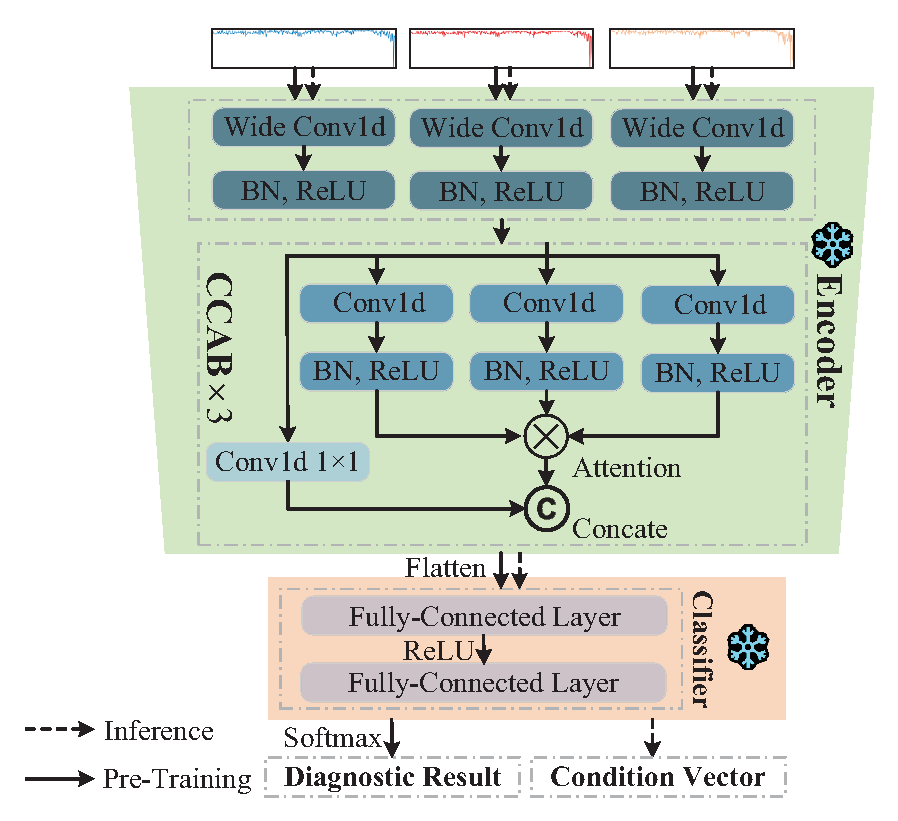
\includegraphics[width=3.3in]{figures/ControlNet.eps}
	\caption{ControlNet的架构。}
	\label{fig_controlnet}
\end{figure}

在反向扩散阶段，外部条件向量$\bm{c}$通过多头注意力机制集成，以确保生成样本的语义一致性。
在第$s$个反向扩散步骤，查询($\bm{Q}^{(s)}$)、键($\bm{K}^{(s)}$)和值($\bm{V}^{(s)}$)表示计算为
\begin{equation}
	\bm{Q}^{(s)} = \bm{W}_{Q}\bar{\bm{x}}_{v}^{(s)},
	\bm{K}^{(s)} = \bm{W}_{K}{\tau}{(\bm{c})},
	\bm{V}^{(s)} = \bm{W}_{V}{\tau}{(\bm{c})},
\end{equation}
其中$\bm{W}_{Q}$、$\bm{W}_{K}$和$\bm{W}_{V}$是可学习的线性投影矩阵，${\tau}{(\cdot)}$表示一个编码器，将$\bm{c}$和$\bar{\bm{x}}_{v}^{(s)}$投影到相同维度的特征空间。
然后注意力输出计算为
\begin{equation}
	\bm{A}^{(s)} = \operatorname{Softmax} \Bigl(\frac{\bm{Q}^{(s)}\bigl({\bm{K}}^{(s)}\bigr)^{\!\top}}{\sqrt{d_{k}}}\Bigr){\bm{V}}^{(s)},
\end{equation}
其中$d_k$是键的维度。
在多头注意力框架中，注意力过程在多个头上独立应用。
每个头的输出然后被拼接并通过线性变换投影以产生最终输出，表示为
\begin{equation}
	\operatorname{MHA}\bigl(\bar{\bm{x}}_{v}^{(s)},\bm{c}\bigr)=
	\bm{W}_{o}\bigl[\bm{A}^{(s)}_{1};\dots;\bm{A}^{(s)}_{N_h}\bigr],
\end{equation}
其中$\bm{W}_{o}$是输出投影矩阵，$N_h$表示注意力头的数量。
通过以这种方式集成外部条件向量$\bm{c}$，我们有效地将语义上下文注入反向扩散过程的每一步。

设计的ControlNet引导跨数据集条件扩散模型的损失函数可表示为
\begin{equation}
	L^{(s)}=\mathbb{E}_{\substack{s\sim[1,S],\bm{x}_v^{(s)},\epsilon^{(s)}}}
	\Bigl[\operatorname{Huber}\bigl(\lVert r^{(s)} \bigr)\rVert\bigr)\Bigr],
\end{equation}
其中$r^{(s)} = \bigl\lVert\epsilon^{(s)} - \epsilon_{{\theta}_\mathrm{d}}\!\bigl(\bar{\bm{x}}_{v}^{(s)},s,\bm{c}\bigr)\bigr\rVert$，$\operatorname{Huber}(\cdot)$是Huber损失。
Huber损失衰减大点态残差的影响，因此对信号样本之间可能存在的相位偏移更加鲁棒，其展开式为
\begin{equation}
	\operatorname{Huber}\bigl(r^{(s)}\bigr)=
	\begin{cases}
		\dfrac{1}{2}\, \bigl(r^{(s)}\bigr)^{2},          & r^{(s)} < \lambda ,\\[4pt]
		\lambda\,\bigl(r^{(s)}-\dfrac{\lambda}{2}\bigr),   & \text{otherwise},
	\end{cases}
	\label{eq:huber}
\end{equation}
其中$\lambda$是$\operatorname{Huber}(\cdot)$的转移阈值。


\subsection{可信多模态大语言模型}

%符号后续还需要统一细化
TMLLM旨在跨多个数据集提供可信的诊断结果和分析。
在TMLLM中，多模态大语言模型通过在文本-信号对上微调预训练LLM来开发。
为获得可信回答，我们通过计算点二列相关系数并进行显著性检验，定位能量异常下降的关键token。
此外，我们设计了一个关键token驱动的不确定性重加权策略来量化LLM回答中的不确定性。

\subsubsection{基于文本-信号对微调LLM}
由于最近的预训练LLM针对离散文本token进行优化，无法原生处理振动信号，我们引入了一个双分支tokenizer-编码器块，将振动信号样本和相应的文本描述转换为信号特定和token特定的特征。
模态特定特征随后通过文本-信号对齐块进行对齐，整个模型被微调以最大化跨模态对齐。

在开发的双分支tokenizer-编码器块中，编码器与ControlNet共享权重$\bm{\theta}_\mathrm{enc}$。
令$\bm{x}_{g}$为合成样本，编码器分支的输入可表示为
$\bm{H}_{g} = \bigl[\bm{x}_{g},\;\tilde{\bm{x}}_{g},\;\bm{x}_{gr}\bigr] \in \mathbb{R}^{3 \times L_{f}}$，其中$\bm{x}_{g}$是查询样本，$\tilde{\bm{x}}_{g}$是无故障信号样本，$\bm{x}_{gr}=\bm{x}_{g}-\tilde{\bm{x}}_{g}$是放大故障相关偏差的残差样本。
该编码器为每个输入产生信号特定特征。
令$\bm{D}=\{k_{1},\dots,k_{N_c}\}$为短文本故障描述的集合，每个故障类别一个描述，其中$N_c$表示类别数。
此外，TMLLM的多模态输入通过融合$\bm{H}_{g}$和$\bm{T}$获得，表示为$\bm{M}_{g}=\{\bm{H}_{g},\bm{T}\}$。
在tokenizer分支中，我们将$\bm{D}$通过LLM的原生tokenizer $\operatorname{Tok}(\cdot)$和嵌入层$\operatorname{Emb}(\cdot)$以获得token特定特征序列，表示为$\bm{E}=\operatorname{Emb}(\operatorname{Tok}(\bm{D})) \in \mathbb{R}^{\gamma\times N_c\times h}$，其中$h$是$\operatorname{Emb}(\cdot)$的隐藏大小，$\gamma$是token特定特征的最大长度。
如图\ref{fig_framework}所示，双分支tokenizer-编码器块的权重在LLM微调期间保持冻结。

为弥合信号特定/token特定特征与LLMs之间的差距，我们开发了一个可训练的文本-信号对齐块，将信号特定和token特定特征融合为适合LLM输入的语言token。
对齐块实现为一个三层线性多层感知器。
我们使用ControlNet的先验权重和token特定特征的组合来初始化该对齐模块。
具体来说，前两个线性层的权重，表示为$\bm{\theta}_\mathrm{l_{1}}$和$\bm{\theta}_\mathrm{l_{2}}$，使用ControlNet预训练分类器的权重$\bm{\theta}_\mathrm{cla}$进行初始化。
此外，我们展平$\bm{E}$的最后两个维度，并将所得矩阵用作$l_{3}$的权重，表示为
$\boldsymbol{\theta}_{l_{3}} =\operatorname{reshape}\bigl(\bm{E},(\gamma,N_c h)\bigr)
\in\mathbb{R}^{\gamma\times N_c h}$。
这样，$\boldsymbol{\theta}_{l_{3}}$的第$i$行编码了第$i$个故障描述的token级嵌入，提供了从信号特定特征到语言token的语义投影。
最后，文本-信号对齐块将语言token嵌入预定义的提示模板中，并输出$\bm{x}_{pt}$作为LLM的输入。
文本-信号对齐块的权重表示为$\boldsymbol{\theta}_\mathrm{ts}=\{\bm{\theta}_\mathrm{l_{1}}, \bm{\theta}_\mathrm{l_{2}}, \bm{\theta}_\mathrm{l_{3}}\}$，预训练LLM的权重表示为$\boldsymbol{\theta}_\mathrm{llm}$。
为了在下游任务上微调文本-信号对齐块和LLM的权重，我们采用使用低秩适配(LoRA)\cite{20231213775448}的参数高效方法。

\subsubsection{关键token定位}
为解决序列级幻觉的隐蔽性问题，我们联合考虑自回归生成规则和诊断特定特征。
% We hypothesize that key tokens exist that act as sentinel positions that expose imminent uncertainty.
我们假设某些关键token充当哨兵，发出即将发生不确定性的信号。
然后，我们在保留语料库上进行点二列相关计算来评估该假设，比较幻觉回答之前token的能量与事实回答中匹配token的能量。
最后，我们进行显著性检验以表明能量的下降是由不期望输入引起的，而非随机波动。
显著性检验返回$p=3.2779\times10^{-28}$，拒绝了低能量token随机出现的零假设。

在生成诊断回答时，LLMs通过一次预测一个token来自回归生成回答，并为下一个token产生词汇表上的概率分布，可表示为
\begin{equation}
	P\bigl(\mathit{Token}_{k} = w \;\big|\; \mathit{Token}_{<k}\bigr)
	\;=\;
	\frac{\exp\bigl(\operatorname{Proj}(\bm{a}_{k})_{\,w}\bigr)}
	{\displaystyle \sum_{w' \in \mathcal{V}} 
		\exp\bigl(\operatorname{Proj}(\bm{a}_{k})_{\,w'}\bigr)},
\end{equation}
其中$\mathit{Token}_{k}$是生成步骤$k$的输出token，$\mathit{Token}_{<k}$是$k$之前生成的整个诊断回答token序列，$\mathcal{V}$是LLM的原生词汇表集合，$w$是从$\mathcal{V}$中抽取的单个token，$\bm{a}_{k}$是$k$处的隐藏状态向量，$\operatorname{Proj}(\cdot)$是可学习的线性变换函数，$\sum_{w\in \mathcal{V}} P\bigl(\mathit{Token}_{k} = w \mid \mathit{Token}_{<k}\bigr) = 1$。
当许多token具有较低概率时，表明下一个token预测的不确定性较高。
此外，token的负对数似然(NLL)可解释为token级能量，表示为
\begin{equation}
	\operatorname{NLL}{(\mathit{Token}_{k}=w)}
	=
	-\,\log
	\frac{\exp\bigl(\operatorname{Proj}(\bm{a}_{k})_{\,w}\bigr)}
	{\displaystyle\sum_{w' \in \mathcal{V}}
		\exp\bigl(\operatorname{Proj}(\bm{a}_{k})_{\,w'}\bigr)},
\end{equation}
其中$\operatorname{NLL}{(\cdot)}$是token能量函数。
低NLL表示模型为该token分配了高概率，而高NLL表示LLM在生成此token时存在歧义。

基于这一分析，我们的假设是当LLM首次输出错误的故障分类结果时，token能量在错误分类token周围发生异常变化。
这一假设基于两个事实。
首先，当模型在其回答中输出错误的故障类别时，这是一种严重的幻觉。
其次，上述关于幻觉与能量关系的分析表明，局部幻觉通常伴随着错误附近token能量的异常变化。
%加一句话阐述什么时候升高什么时候降低

为验证我们的假设，我们首先构建一个保留语料库。我们使用MBHM数据集\cite{Peng_Liu_Du_Gao_Wang_2025}的样本作为正常输入，使用MaFaulDa数据集\cite{MaFaulDa_dataset}的样本作为不期望输入，并使用Qwen-2 1.5B模型\cite{QWEN}作为LLM。
% For normal inputs and undesired input, we generate $N_\mathrm{nor}$ and $N_\mathrm{un}$ answers, respectively.
我们为正常输入生成$N_\mathrm{nor}$个回答，为不期望输入生成$N_\mathrm{un}$个回答。
此外，在首次误分类发生的token为中心的$\pm L_{\mathrm{win}}$token窗口内计算token能量，该token表示为$\mathit{Token}_{{\delta}}$。
然后，计算点二列相关系数，表示为$r_\mathrm{pb}$，以检验token能量与相应输入之间的关系。
点二列相关是适用于特殊情况的Pearson相关，量化二进制输入类型与连续token能量之间的相关性。
$r_\mathrm{pb}$表示为
\begin{equation}
	r_\mathrm{{pb}}=
	\frac{\mu_\mathrm{nor} - \mu_\mathrm{un}}{\sigma_\mathrm{total}}
	\sqrt{\frac{N_\mathrm{nor}\,N_\mathrm{un}}{(N_\mathrm{nor}+N_\mathrm{un})^2}},
\end{equation}
其中$\mu_\mathrm{nor}$是正常输入回答的平均token能量，$\sigma_\mathrm{total}$是所有回答token能量的标准差。
最后，我们进行显著性检验来评估$r_\mathrm{pb}$的结果，以表明能量的上升是由不期望输入引起的，而非随机波动。
系数$r_{pb}$被转换为$t$统计量，表示为
\begin{equation}
	t=r_\mathrm{pb}\sqrt{\frac{(N_\mathrm{nor}+N_\mathrm{un}) - 2}{1 - r_\mathrm{pb}^2}},\,\mathrm{df} = (N_\mathrm{nor}+N_\mathrm{un}) - 2, 
\end{equation}
其中$\mathrm{df}$是自由度。
此外，双侧$p$值，表示为$p_{\text{two-sided}}$，然后从学生$t$分布的累积分布函数(CDF)中获得，表示为
\begin{equation}
	p_{\text{two-sided}} = 2\bigl[1-F_{t_{\mathrm{df}}}(|t|)\bigr]
	= 2P\bigl(T_{\mathrm{df}}\ge |t|\bigr),
	\label{eq:p_value}
\end{equation}
其中$F_{t_{\mathrm{df}}}(\cdot)$是自由度为$\mathrm{df}$的学生$t$分布的CDF，$T_{\mathrm{df}}$是服从该分布的随机变量。


如图\ref{fig_correlation}所示，我们在以$\mathit{Token}_{\delta}$为中心的$\pm L_{\mathrm{win}}=3$范围内计算二进制输入类型与token能量序列之间的$r_{\mathrm{pb}}$和$p_{\text{two-sided}}$。
在token $\mathit{Token}_{\delta-1}$处，观察到大的效应量，其中$|r_{\mathrm{pb}}| > 0.5$且$r_{\mathrm{pb}} < -0.5$。
该观察表明token能量的异常下降对不期望输入具有高度预测性。
此外，显著性检验返回$p=3\times10^{-28}$，拒绝了低能量token随机出现的零假设。
从理论角度来看，不期望输入倾向于在$\mathit{Token}_{\delta}$周围诱导局部能量扭曲。
因为${\delta}-1$紧邻${\delta}$，它对不期望输入的最早迹象本质上更具响应性，与统计证据一致。
因此，我们采用$\mathit{Token}_{\delta-1}$作为不期望输入检测的关键token，尽管$\mathit{Token}_{\delta+2}$具有更高的相关性，但将其省略。


\begin{figure}[!t]
	\centering
	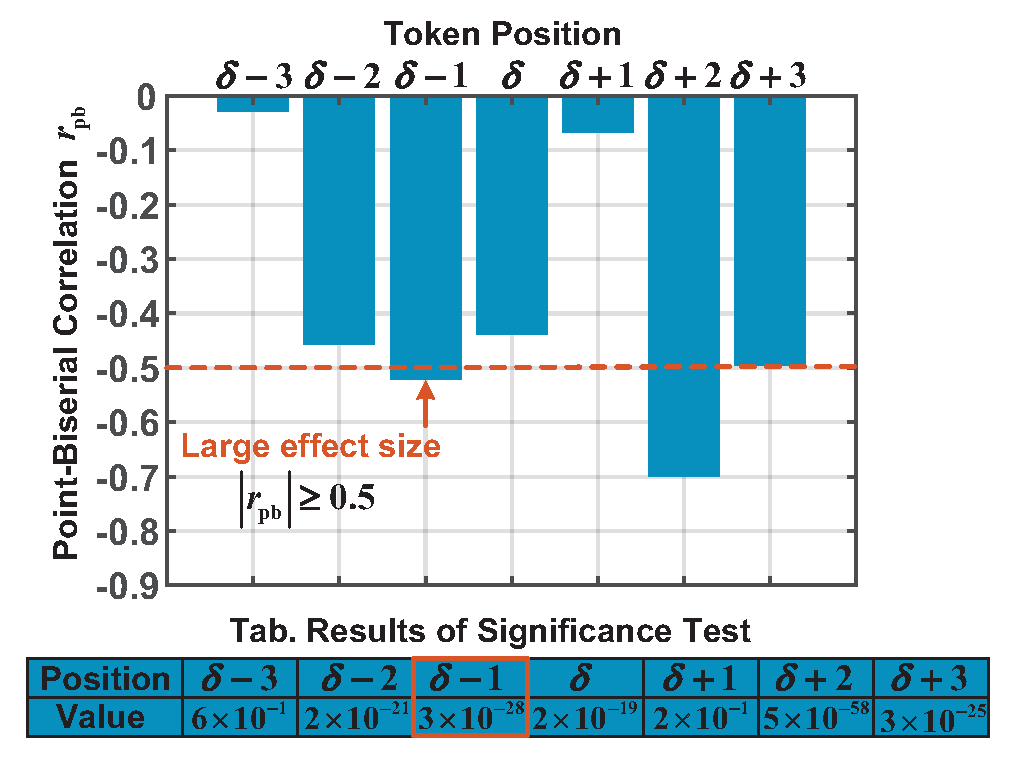
\includegraphics[width=3.5in]{figures/correlation.eps}
	\caption{在以$\mathit{Token}_{\delta}$为中心的$\pm L_{\mathrm{win}}$范围内，二进制输入类型与token能量序列之间的点二列相关系数$r_{\mathrm{pb}}$和双侧$p$值$p_{\text{two-sided}}$。基于理论基础和统计证据，选择$\mathit{Token}_{\delta-1}$作为不期望输入检测的关键token。}
	\label{fig_correlation}
\end{figure}



\subsubsection{关键token驱动的不确定性重加权策略}
为量化LLM输出的不确定性并构建TMLLM，我们提出了关键token驱动的不确定性重加权策略(KTURS)。
所提出的策略采用token级能量作为不确定性量化指标，并为与指定关键token表现出更强相关性的token分配更大的权重。


对于关于多模态输入$\bm{x}_{pt}$的LLM输出$\bm{\hat y}_{g}$，表示为$\bm{\hat y}_{g}=\{\mathit{Token}_{1},\mathit{Token}_{2},\dots,\mathit{Token}_{N_t}\}$，其中$N_t$是输出长度。
我们首先为每个token $\mathit{Token}_{k} (1\leq k\leq N_t)$计算归一化能量分数，表示为
\begin{equation}
	\label{equa:normalized_energy_score}
	\begin{split}
		{\operatorname{\tilde{NLL}}}(\mathit{Token}_k)
		= \,\frac{{\operatorname{NLL}}(\mathit{Token}_k)}
		{\sum_{j=1}^{N_t}{{\operatorname{NLL}}(\mathit{Token}_j)}\,}\,.
	\end{split}
\end{equation}
然后，我们根据$r_\mathrm{pb}$通过放大关键token的权重来推导token级不确定性，表示为
\begin{equation}
	\label{equa:token_level_uncertainty}
	\begin{split}
		&\operatorname{UT}(\mathit{Token}_k;\omega,r_{\mathrm{pb}})\\
		&= \bigl[1 + (\omega r_{\mathrm{pb}} - 1)\bm{1}_{\{k=\delta-1\}}\bigr]
		\tilde{\operatorname{NLL}}(\mathit{Token}_k),
	\end{split}
\end{equation}
其中$\bm{1}_{\{k=\delta-1\}}$当token索引$k=\delta-1$时为1，否则为0，$\omega$是用于校准token级不确定性程度的系数。
最后，LLM输出的不确定性可表示为
\begin{equation}
	\label{equa:overall_uncertainty}
	\operatorname{UA}(\bm{\hat y}_{g})
	= \sum_{k=1}^{N_t}
	\bigl[\,1 + (\omega\,r_{\mathrm{pb}} - 1)\,\bm{1}_{\{k=\delta-1\}}\,\bigr]\;\tilde{\operatorname{NLL}}(\mathit{Token}_k)\,.
\end{equation}


如图\ref{fig_strategy}所示，原始能量分数首先被归一化为不确定性分布
$\tilde{\operatorname{NLL}}(\mathit{Token}_k)$，然后关键token $\mathit{Token}_{\delta}$的不确定性被因子$\omega$放大，最后通过对所有$N_t$个token的token级不确定性求和获得序列级不确定性$\operatorname{UT}(\mathit{Token}_k;\omega,r_{\mathrm{pb}})$。

\begin{figure}[!t]
	\centering
	
\includegraphics[width=3.5in]{figures/whole_strategy.eps}
	\caption{关键token驱动的不确定性重加权策略示意图。}
	\label{fig_strategy}
\end{figure}


\subsection{基于DA-TMLLM的抗幻觉方案}
\label{sec:scheme}
为缓解和检测LLM幻觉，所提出的抗幻觉方案将基于扩散的增强和可信多模态大语言模型整合到一个统一的流程中。

为缓解统计偏差诱导的幻觉，ControlNet引导的跨数据集条件扩散模型被设计用于产生平衡且语义对齐的合成数据。
原始样本和合成样本随后被融合并用于微调可信多模态大语言模型。  
训练阶段的流程总结在算法\ref{alg:training}中。
在输入任何测试样本之前，我们在仅包含正常样本的验证集上评估不确定性分数的均值和方差，表示为$\mu_\mathrm{val}$和$\sigma_\mathrm{val}$。 
这使我们能够定义不确定性阈值的上下界，$\psi_{lower}=\mu_\mathrm{val} - \sigma_\mathrm{val}$和$\psi_{upper}=\mu_\mathrm{val} + \sigma_\mathrm{val}$，它们共同形成决策区间$[\psi_{lower}, \psi_{upper}]$。
此外，我们定位关键token并设计关键token驱动的不确定性重加权策略。
推理阶段的流程总结在算法\ref{alg:inference}中。

\begin{algorithm}[t]
	\caption{扩散增强可信多模态大语言模型的训练流程}
	\label{alg:training}
	\centering
	\begin{algorithmic}[1]
		\Require 预处理数据集$\mathcal{D}_\text{real}=\{(\mathbf{x}_{v},y)\}$，权重$\bm{\theta}_\mathrm{enc}$、${\theta}_\mathrm{d}$、$\bm{\theta}_\mathrm{cla}$、$\bm{\theta}_\mathrm{ts}$和$\bm{\theta}_\mathrm{llm}$，超参数$S$、$N_\mathrm{dm}$、$N_\mathrm{llm}$和$N_{\text{aug}}$，响应文本$\bm{y}_{g}$
		\Ensure 训练好的CGCDM $\bm{\theta}_\mathrm{d}^*$，微调后的TMLLM $\bm{\theta}_\mathrm{ts}^*$、$\bm{\theta}_\mathrm{llm}^*$
		\Statex \textbf{阶段1：训练ControlNet引导的CDM}
		\For{epoch $=1$ \textbf{to} $N_\mathrm{dm}$} \Comment{训练轮数$N_\mathrm{dm}$}
		\ForAll{$(\bm{x}_{v},y)\!\sim\!\mathcal{D}_\text{real}$}
		\State $\bm{x}_{v}^{(S)}\leftarrow\textsc{AddNoise}(\bm{x}_{v},S)$
		\State $L^{(s)}\!\leftarrow\!\lVert\epsilon-\epsilon_{\bm{\theta}_\mathrm{d}}(\bm{x}_{v}^{(s)},y,s)\rVert_2^2$
		\State $\bm{\theta}_\mathrm{d}^*\!\leftarrow\!\bm{\theta}_\mathrm{d}-\eta_{\bm{\theta}_\mathrm{d}}\nabla_{\bm{\theta}_\mathrm{d}}L^{(s)}$
		\EndFor
		\EndFor
		\Statex \textbf{阶段2：生成增强样本}
		\For{$n=1$ \textbf{to} $N_{\text{aug}}$} \Comment{增强样本数$N_{\text{aug}}$}
		\State $\bm x_{v}^{(S)}\sim\mathcal N(\bm 0,\bm I)$ 
		\For{$s=S$ \textbf{downto} $1$}
		\State $\bm c\leftarrow\textsc{ControlNet}(\bm{\theta}_\mathrm{enc}, \bm{\theta}_\mathrm{cla})$
		\State $\bm\mu\leftarrow\textsc{PosteriorMean}(\bm x^{(s)},s,\bm c,\bm{\theta}_\mathrm{d}^*)$
		\State $\bm\bar{\bm x}_{v}^{(s-1)}\sim\mathcal N\!\bigl(\bm\mu,(\sigma^{(s)})^{2}\bm I\bigr)$
		\EndFor
		\State $\mathcal D_{\text{syn}}\gets\mathcal D_{\text{syn}}\cup\{\bar{\bm{x}}_v^{(0)}\}$
		\EndFor
		\State $\mathcal{D}_\text{aug}\!\leftarrow\!\mathcal{D}_\text{real}\cup\mathcal{D}_\text{syn}$
		\Statex \textbf{阶段3：微调可信多模态大语言模型}
		\State 初始化${\bm{x}}_g\!\leftarrow\!\bar{\bm{x}}_v$
		\For{epoch $=1$ \textbf{to} $N_\mathrm{llm}$} \Comment{训练轮数$N_\mathrm{llm}$}
		\ForAll{$(\bm{x}_{g},\bm{y}_{g})\!\sim\!\mathcal{D}_\text{aug}$}
		\State $\bm{x}_{pt}\leftarrow\textsc{AlignBlock}(\bm{x}_{g})$
		\State $\bm{\hat y}_{g}\leftarrow\textsc{TMLLM}(\bm{x}_{pt})$
		\State $\bm{\theta}_\mathrm{ts}^*, \bm{\theta}_\mathrm{llm}^*\leftarrow \operatorname{LoRA}(\bm{\hat y}_{g}, \bm{y}_{g})$
		\EndFor
		\EndFor
		\State \Return $\bm{\theta}_\mathrm{d}^*$、 $\bm{\theta}_\mathrm{ts}^*$、$\bm{\theta}_\mathrm{llm}^*$
	\end{algorithmic}
\end{algorithm}

\begin{algorithm}[t]
	\caption{基于关键token驱动不确定性重加权策略的推理流程}
	\label{alg:inference}
	\begin{algorithmic}[1]
		\Require 测试集$\mathcal{D}_\text{test}$，窗口长度$L_{\mathrm{win}}$，TMLLM权重$\bm{\theta}_\mathrm{ts}^*$、$\bm{\theta}_\mathrm{llm}^*$，校准系数$\omega$，关键token索引$\delta-1$，不确定性阈值$\psi$
		\ForAll{$\bm{x}_\mathrm{test}\!\sim\!\mathcal{D}_\mathrm{test}$}
		\State $\hat{\bm{y}}_\mathrm{test} \gets \mathrm{TMLLM}(\bm{\theta}_\mathrm{ts}^*$, $\bm{\theta}_\mathrm{llm}^*;\bm{x}_\mathrm{test})$
		\State $\hat{\bm{y}}_\mathrm{test}=\{\mathit{Token}_1,\dots,\mathit{Token}_{N_t}\}$
		\Statex \textbf{阶段1：Token级归一化}
		\For{$k = 1$ \textbf{to} $N_t$}
		\State $\operatorname{NLL}_k \gets -\!\log P\!\bigl(\mathit{Token}_k \mid \mathit{Token}_{<k}\bigr)$
		\EndFor
		\State $\displaystyle
		\tilde{\operatorname{NLL}}_k \gets 
		\operatorname{NLL}_k \Big/ \sum_{j=1}^{N_t}\operatorname{NLL}_j$
		\Statex \textbf{阶段2：关键token重加权}
		\For{$k = 1$ \textbf{to} $N_t$}
		\State $\displaystyle
		\operatorname{UT}_k \gets
		\Bigl[1 + \bigl(\omega r_{\mathrm{pb}} - 1\bigr)\,
		\mathbf{1}_{\{k=\delta-1\}}\Bigr]\!
		\tilde{\operatorname{NLL}}_k$
		\EndFor
		\Statex \textbf{阶段3：序列级聚合}
		\State $\displaystyle
		\operatorname{UA}\!\bigl(\hat{\bm{y}}_\mathrm{test}\bigr) \gets
		\sum_{k=1}^{N_t}\operatorname{UT}_k$
		\Statex \textbf{阶段4：决策}
		\If{$\operatorname{UA}\!\bigl(\hat{\mathbf{y}}_{\text{test}}\bigr)\not\in[\psi_{lower}, \psi_{upper}]$}
		\State \textbf{拒绝} $\bm{x}_\mathrm{test}$ \Comment{检测到幻觉}
		\Else
		\State \textbf{输出} $\hat{\bm{y}}_\mathrm{test}$
		\EndIf
		\EndFor
	\end{algorithmic}
\end{algorithm}
%

\section{实验}
本节对DA-TMLLM进行了全面评估，在十一个数据集和七个评估指标上将其与九个基线方法进行了基准比较。
首先，我们在幻觉易发场景下评估DA-TMLLM的性能，并评估数据增强对少数类的有效性。
其次，进行消融研究以量化每个关键组件的贡献。
第三，我们分析DA-TMLLM性能对不同超参数的敏感性。

\subsection{实验设置}
为了在幻觉易发场景下对DA-TMLLM与对比模型进行基准测试，我们采用两类数据集：域特定数据集和不期望数据集。
不期望数据集仅在测试阶段使用，用于构建不期望测试子集，以量化模型拒绝不期望输入的能力。
域特定数据集由多个轴承数据集组成，被划分为训练集、验证集和域特定测试子集。
此外，我们将域特定测试子集和不期望测试子集合并为复合测试集，以对模型的抗幻觉性能进行统一评估。
域特定数据集包括九个轴承数据集：PU\cite{PU}、JNU\cite{s130608013}、CWRU\cite{15467457}、JUST\cite{JUST}、DIRG\cite{DAGA2019252}、HIT\cite{HIT}、IMS\cite{IMS}、MFPT\cite{MFPT}和XJTU\cite{XJTU}，所有这些数据集都包含在MBHM仓库\cite{Peng_Liu_Du_Gao_Wang_2025}中。
% The details of domain-specific datasets are presented in Table \ref{tab:Detailed datasets}, including their fault location-characterized data type and the corresponding number of samples.
% Table \ref{tab:Detailed datasets} overviews the nine domain-specific bearing datasets employed, listing the fault-location classes and the corresponding sample counts for each dataset.
表\ref{tab:Detailed datasets}总结了本研究中使用的九个域特定轴承数据集，详细列出了各自的故障位置类别和样本数量。
不期望数据集由UP\cite{UP_dataset}和MaFaulDa\cite{MaFaulDa_dataset}数据集组成。

\setlength{\tabcolsep}{5pt}
\begin{table*}[!htbp]
	\footnotesize
	% table caption is above the table
	\caption{数据集概览}
	\centering
	\label{tab:Detailed datasets} % Give a unique label
	% For LaTeX tables use
	\begin{tabular}{lccccccccccc} % 10 列
		\toprule[1pt]\noalign{\smallskip}
		故障位置 & PU & JNU & CWRU & JUST & DIRG & HIT & IMS & MFPT & XJTU &总样本数& 训练样本数\\
		& \cite{PU} & \cite{s130608013} & \cite{15467457} & \cite{JUST} & \cite{DAGA2019252} & \cite{HIT} & \cite{IMS} & \cite{MFPT} & \cite{XJTU} &&\\
		\noalign{\smallskip}\hline\noalign{\smallskip}
		无故障 (FF)& 1918 & 900 & 70 & 10932 & 1020 & 3816 & 43176 & 18 & 11014 & 72864 & 10000\\
		\noalign{\smallskip}\hline\noalign{\smallskip}
		轻微内圈故障 (MiIR)& 954 & - & 310 & - & 1020 & - & 812 & - & 64 & 3160 &2736\\
		\noalign{\smallskip}\hline\noalign{\smallskip}
		中度内圈故障 (MoIR)& 633 & 900 & 296 & 11124 & 1020 & 4032 & - & 21 & 28 & 18054 &10000\\
		\noalign{\smallskip}\hline\noalign{\smallskip}
		严重内圈故障 (SIR)& -\textsuperscript{1} & - & 350 & - & 1020 & - & - & - & 232 & 1602 &345\\
		\noalign{\smallskip}\hline\noalign{\smallskip}
		轻微滚珠故障 (MiB)& - & - & 310 & - & 1020 & - & - & - & 30 & 1360 &45\\
		\noalign{\smallskip}\hline\noalign{\smallskip}
		中度滚珠故障 (MoB)& - & 900 & 310 & 10956 & 1020 & - & 1000 & - & 60 & 14246 &10000\\
		\noalign{\smallskip}\hline\noalign{\smallskip}
		严重滚珠故障 (SB)& - & - & 350 & - & 1020 & - & 312 & - & 356 & 2038 &1005\\
		\noalign{\smallskip}\hline\noalign{\smallskip}
		轻微外圈故障 (MiOR)& 2223 & - & 918 & - & - & - & 575 & - & 284 & 4000 & 4620 \\
		\noalign{\smallskip}\hline\noalign{\smallskip}
		中度外圈故障 (MoOR)& 1588 & 900 & 340 & 10974 & - & 1800 & 447 & 39 & 260 & 16348 &10000\\
		\noalign{\smallskip}\hline\noalign{\smallskip}
		严重外圈故障 (SOR)& - & - & 678 & - & - & - & 158 & - & 1008 & 1844 &1764\\
		\noalign{}\bottomrule[1pt]
		\multicolumn{10}{l}{\textsuperscript{1} 破折号(–)表示该数据集中不存在相应的故障位置类别。}\\[-5pt]
	\end{tabular}
\end{table*}


\setlength{\tabcolsep}{6pt}

为评估模型对由统计偏差引起的幻觉的鲁棒性，我们在训练和验证期间遵循\cite{20243817051432}的极端类别不平衡设置，其中最大类和最小类之间的比率超过100。
此外，我们采用平衡的域特定测试子集，使每个类别对诊断性能的贡献相等。 
MaFaulDa数据集包含与域特定数据集具有高语义相似性的轴承振动信号。
相比之下，UP数据集包含水下螺旋桨故障信号，在运行环境和信号特征上都表现出显著的域偏移。
为评估模型对不同程度相似性不期望输入诱导幻觉的抵抗能力，定义了三种类型的复合测试场景。
场景1使用由域特定子集与UP组合形成的测试集。
场景2用MaFaulDa替换UP，确保与训练数据集的高语义相似性。
场景3采用由域特定子集、UP和MaFaulDa组成的复合测试集，产生混合域评估设置。

\begin{table}[h!]
	\footnotesize
	\caption{超参数设置}
	\centering
	\label{tab:Hyperparameter}       % Give a unique label
	% For LaTeX tables use
	\begin{tabular}{lll}
		\toprule[1pt]\noalign{}
		符号&描述&值 \\
		\noalign{}\hline\noalign{\smallskip}
		$L_{f}$&样本长度& $2400$ \\
		$\rho$&$\operatorname{SNorm}(\cdot)$的缩放因子& $0.01$ \\
		$S$&扩散步数& $10$ \\
		$\zeta$ & 扩散模型的噪声调度器 & $Linear$ \\
		$N_{h}$&注意力头数& $4$ \\
		$N_{c}$&样本类别数& $10$ \\
		$\lambda$&$\operatorname{Huber}(\cdot)$的转移阈值& $1$ \\
		$N_{t}$& 输出token的最大长度 & $2048$ \\
		$\mathcal{M}_{tune}$ & 微调的目标模块 & $all\_linear$\\
		$r_{LoRA}$ & LoRA微调的秩 & 4 \\
		$L_{\mathrm{win}}$&token窗口长度& $\pm 3$ \\
		$\omega$&关键token的校准系数& $50$ \\
		$n_{diff}$&扩散的批次大小& $32$ \\
		$n_{tune}$&微调的批次大小 & $1$ per GPU\\
		${N_\mathrm{dm}}$&CGCDM的训练轮数& $100$ \\
		${N_\mathrm{llm}}$&TMLLM的训练轮数& $50$ \\
		${n_{lr}}$&学习率& $1 \times 10^{-4}$ \\
		${n_{dr}}$&Dropout率& $0.1$ \\
		\bottomrule[1pt]
	\end{tabular}
\end{table}

所有评估均在使用NVIDIA RTX 4090 GPU的工作站上使用PyTorch进行。
15亿参数的Qwen2\cite{QWEN}模型作为基础LLM，采用LoRA技术\cite{20231213775448}对TMLLM进行微调。
DA-TMLLM的超参数总结在表\ref{tab:Hyperparameter}中。
此外，数据集特定的采样率$\nu$在相应的数据集文档中提供。
使用八个指标对DA-TMLLM和对比模型进行全面评估，其中$\uparrow$表示较大值表示性能更优，$\downarrow$表示较低值更优。

\textit{域特定准确率} (DS-ACC, $\uparrow$) 计算正确诊断的故障类型与来自域特定测试子集的样本总数的比率。

\textit{总体准确率} (G-ACC, $\uparrow$) 呈现在结合域特定和不期望样本的混合测试集上的总体诊断准确率。

\textit{受试者工作特征曲线下面积} (AUROC, $\uparrow$) 测量域特定样本和不期望样本之间的可分离性，较高值表示更强的分离能力。

\textit{95\%召回率下的误报率} (FAR@95, $\downarrow$) 是当检测器达到95\%不期望召回率时，被错误分类为不期望样本的域特定样本比例。

\textit{精确率-召回率曲线下面积} (AUPR, $\uparrow$) 强调域特定准确率，较高值表示更干净地拒绝不期望样本。

\textit{均方根误差} (RMSE, $\downarrow$) 通过测量合成信号与实际信号之间点态差异的二次均值来呈现生成质量。

\textit{峰值信噪比} (PSNR, $\uparrow$) 通过测量最大信号功率与损坏噪声功率之比来量化重建质量。

\textit{频谱余弦相似度} (FSCS, $\uparrow$) 通过计算幅度谱的相似度来表达合成信号与实际信号之间的生成质量。

\setlength{\tabcolsep}{1.6pt}
\begin{table*}[t!]
	\footnotesize
	% table caption is above the table
	\caption{抗幻觉故障诊断实验结果\textsuperscript{1}}
	\renewcommand{\arraystretch}{1.5}
	\centering
	\label{tab:comparison result1}       % Give a unique label
	% For LaTeX tables use
	\begin{tabular}{c|ccccc|ccccc|ccccc}
		\toprule[1pt]\noalign{\vspace{0.5pt}}
		场景&\multicolumn{5}{c|}{场景1\textsuperscript{2}}&\multicolumn{5}{c|}{场景2\textsuperscript{3}}&\multicolumn{5}{c}{场景3\textsuperscript{4}}
		\\\cmidrule(lr){2-6}\cmidrule(lr){7-11}\cmidrule(lr){12-16}
		指标&DS-ACC &G-ACC &AUROC &FAR@95 &AUPR &DS-ACC &G-ACC &AUROC &FAR@95 &AUPR &DS-ACC &G-ACC &AUROC &FAR@95 &AUPR \\\midrule[1pt]
		VQVAE & 78.89\% & 72.82\% & 0.6812  & 0.8028  & 0.1490  & 78.89\% & 72.82\% & 0.5832  & 1.0000  & 0.0956  & 78.89\% & 67.62\% & 0.6322  & 0.8083  & 0.2047  \\
		\noalign{\vspace{2.8pt}}\hline\noalign{\smallskip}
		DCGAN & 85.56\% & 78.97\% & 0.4596  & 0.7083  & 0.0678  & 85.56\% & 78.97\% & 0.7306  & 0.4861  & 0.1468  & 85.56\% & 73.33\% & 0.5951  & 0.6917  & 0.1730  \\
		\noalign{\vspace{2.8pt}}\hline\noalign{\smallskip}
		QSCGAN & 83.89\% & 77.44\% & 0.5393  & 1.0000  & 0.0942  & 83.89\% & 77.44\% & 0.6821  & 0.6194  & 0.1261  & 83.89\% & 71.90\% & 0.6107  & 0.9139  & 0.1896  \\
		\noalign{\vspace{2.8pt}}\hline\noalign{\smallskip}
		BearLLM & 88.33\% & 81.54\% & 0.5893  & 0.9083  & 0.0983  & 88.33\% & 81.54\% & 0.7328  & 0.7472  & 0.2326  & 88.33\% & 75.71\% & 0.6610  & \underline{0.2545}  & 0.8778  \\
		\noalign{\vspace{2.8pt}}\hline\noalign{\smallskip}
		MLMM  & \underline{89.17\%} & \underline{88.46\%} & 0.9622  & 0.2722  & 0.8660  & 89.17\% & \underline{86.92\%} & 0.9181  & 0.2833  & 0.7464  & \underline{89.17\%} & \underline{86.43\%} & \underline{0.9401}  & 0.2722  & 0.8483  \\
		\noalign{\vspace{2.8pt}}\hline\noalign{\smallskip}
		WDSN  & 71.94\% & 74.10\% & 0.9795  & 0.1000  & 0.9983  & 71.94\% & 72.56\% & 0.8139  & 0.9000  & \textbf{0.9806}  & 71.94\% & 74.29\% & 0.8888  & 0.4667  & \underline{0.9790}  \\
		\noalign{\vspace{2.8pt}}\hline\noalign{\smallskip}
		MDCC  & 77.50\% & 79.23\% & \underline{0.9867}  & \underline{0.0333}  & \underline{0.9989}  & 77.50\% & 81.54\% & 0.7636  & 0.9000  & \underline{0.9749}  & 77.50\% & 78.81\% & 0.8722  & 0.5333  & 0.9735  \\
		\noalign{\vspace{2.8pt}}\hline\noalign{\smallskip}
		LLMCheck & 85.28\% & 73.33\% & 0.5744  & 0.7000  & 0.5189  & 85.28\% & 71.03\% & 0.5567  & 0.6667  & 0.5641  & 85.28\% & 76.19\% & 0.6544  & 0.7500  & 0.5707  \\
		\noalign{\vspace{2.8pt}}\hline\noalign{\smallskip}
		MIND  & 85.00\% & 82.05\% & 0.8611  & 0.6333  & 0.8641  & 85.00\% & 82.82\% & 0.8889  & \underline{0.2667}  & 0.8310  & 85.00\% & 78.57\% & 0.8206  & 0.4500  & 0.8088  \\
		\noalign{\vspace{2.8pt}}\hline\noalign{\smallskip}
		SHalluDetect & \textbf{92.78\%} & 85.64\% & 0.6066  & 1.0000  & 0.9318  & \textbf{92.78\%} & 85.64\% & 0.6289  & 0.7333  & 0.9445  & \textbf{92.78\%} & 79.52\% & 0.5112  & 0.8333  & 0.8581  \\
		\noalign{\vspace{2.8pt}}\hline\noalign{\smallskip}
		LLM-OOD & 85.28\% & 77.69\% & 0.8646  & 0.8038  & 0.8222  & 85.28\% & 78.46\% & \underline{0.9615}  & 0.8870  & 0.4222  & 85.28\% & 78.10\% & 0.9131  & 0.8688  & 0.6944  \\
		\noalign{\vspace{2.8pt}}\hline\noalign{\smallskip}
		DA-TMLLM & \textbf{92.78\%} & \textbf{93.33\% }& \textbf{1.0000}  & \textbf{0.0000}  & \textbf{1.0000}  & \textbf{92.78\%} & \textbf{92.82\%} & \textbf{0.9860}  & \textbf{0.0028}  & 0.9092  & \textbf{92.78\%} & \textbf{93.57\%} & \textbf{0.9942}  & \textbf{0.0000}  & \textbf{0.9887}  \\
		\noalign{\vspace{0.5pt}}
		\bottomrule[1pt]
		\multicolumn{13}{l}{\textsuperscript{1} 最佳结果：\textbf{粗体}；次佳结果：\underline{下划线}。}\\	[-5pt]
		\multicolumn{13}{l}{\textsuperscript{2} 场景1使用由域特定子集与UP组合形成的测试集。}\\	[-5pt]
		\multicolumn{13}{l}{\textsuperscript{3} 场景2用MaFaulDa替换UP，确保与训练数据集的高语义相似性。}\\	[-5pt]
		\multicolumn{16}{l}{\textsuperscript{4} 场景3采用由域特定子集、UP和MaFaulDa组成的复合测试集，产生混合域评估设置。}\\	[-5pt]
	\end{tabular}
\end{table*}
\setlength{\tabcolsep}{6pt}

\subsection{性能对比}

我们在MBHM、MaFaulDa和UP数据集上评估了DA-TMLLM和十一个基线模型的抗幻觉故障诊断性能。表\ref{tab:comparison result1}展示了使用五个指标(包括DS-ACC、G-ACC、AUROC、FAR@95和AUPR)在场景1、2和3中的结果。实验结果突显了DA-TMLLM的优越性，它大幅且始终优于所有基线模型。在场景1中，我们的模型在DS-ACC和G-ACC上分别比次佳模型提高了4.05\%和5.51\%，同时达到了理想的检测性能。这种优势在场景3的复杂混合域设置中得以保持，再次在所有指标上取得了最先进的结果。唯一的例外是在场景2中，DA-TMLLM在AUPR指标上略逊于WDSN。尽管如此，它仍在G-ACC上领先，并在FAR@95上实现了相比最近基线98.95\%的降低。平均而言，相比最强竞争对手，G-ACC提高了6.85\%，FAR@95降低了99.65\%，DA-TMLLM有效展示了其同时执行高精度故障诊断和鲁棒幻觉检测的能力。相比之下，基线模型表现出局限性。VQVAE、DCGAN、QSCGAN和BearLLM由于缺乏明确的幻觉检测能力，无法可靠地区分域特定输入和不期望输入，这从DS-ACC到G-ACC的急剧下降以及较差的AUROC和AUPR分数可以看出。在具有检测能力的基线中，可以观察到性能权衡。CDLMs(包括MLMM、WDSN和MDCC)通常在幻觉检测方面更为擅长。相反，基于LLM的方法(包括LLMCheck、MIND、SHalluDetect和LLM-OOD)在分布内分类方面表现出优越性。两类模型都倾向于将有效的域特定样本错误分类为不期望样本，同时在处理被标记为幻觉的输入时过于保守。

为说明跨不同决策阈值的抗幻觉诊断性能，我们绘制了受试者工作特征(ROC)曲线和精确率-召回率(PR)曲线，如图\ref{fig:Performance_Comparison_2}所示。这些可视化从图形上证实了表\ref{tab:comparison result1}中的定量发现。DA-TMLLM的ROC曲线在所有场景中都始终占据理想的左上角，表明卓越的可分离性，这与其AUROC和FAR@95分数一致。类似地，PR曲线显示我们的模型最接近右上角，在召回率范围内保持极高的精确率，证实了其AUPR值。相比之下，基线模型的曲线明显较差，强化了DA-TMLLM实现更鲁棒和可靠幻觉检测的结论。

\begin{figure*}[htbp]
	\centering
	\subfloat[三种场景下的ROC曲线]{
		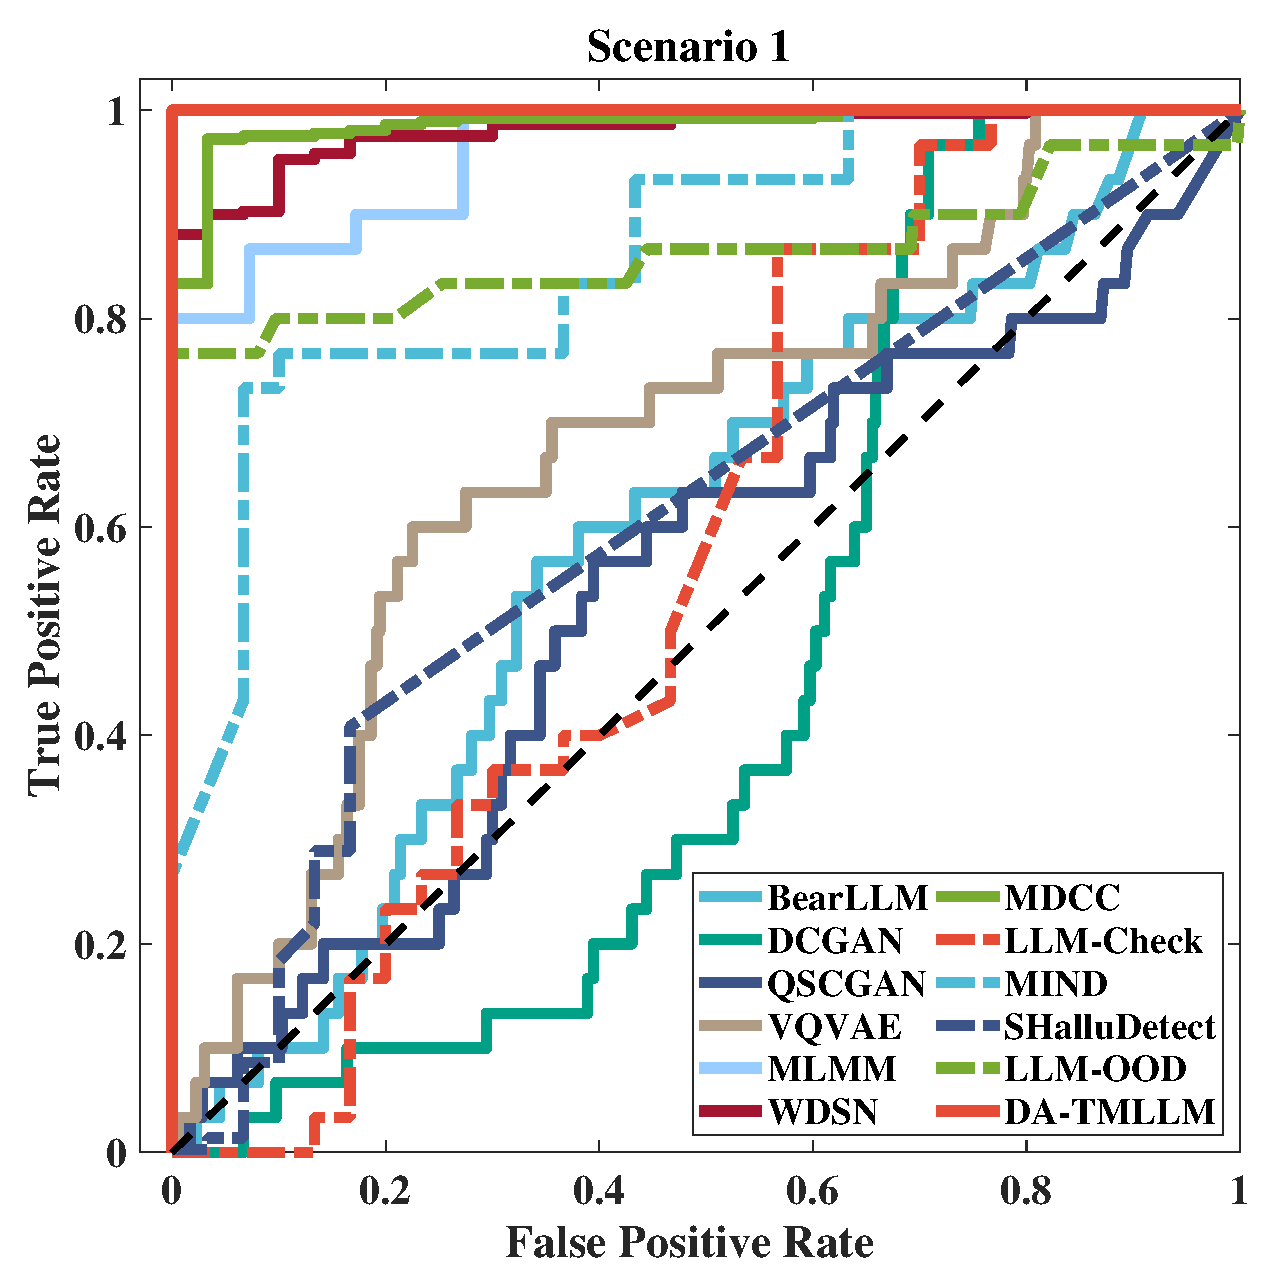
\includegraphics[width=2.3in]{figures/ROC_s1.eps}
		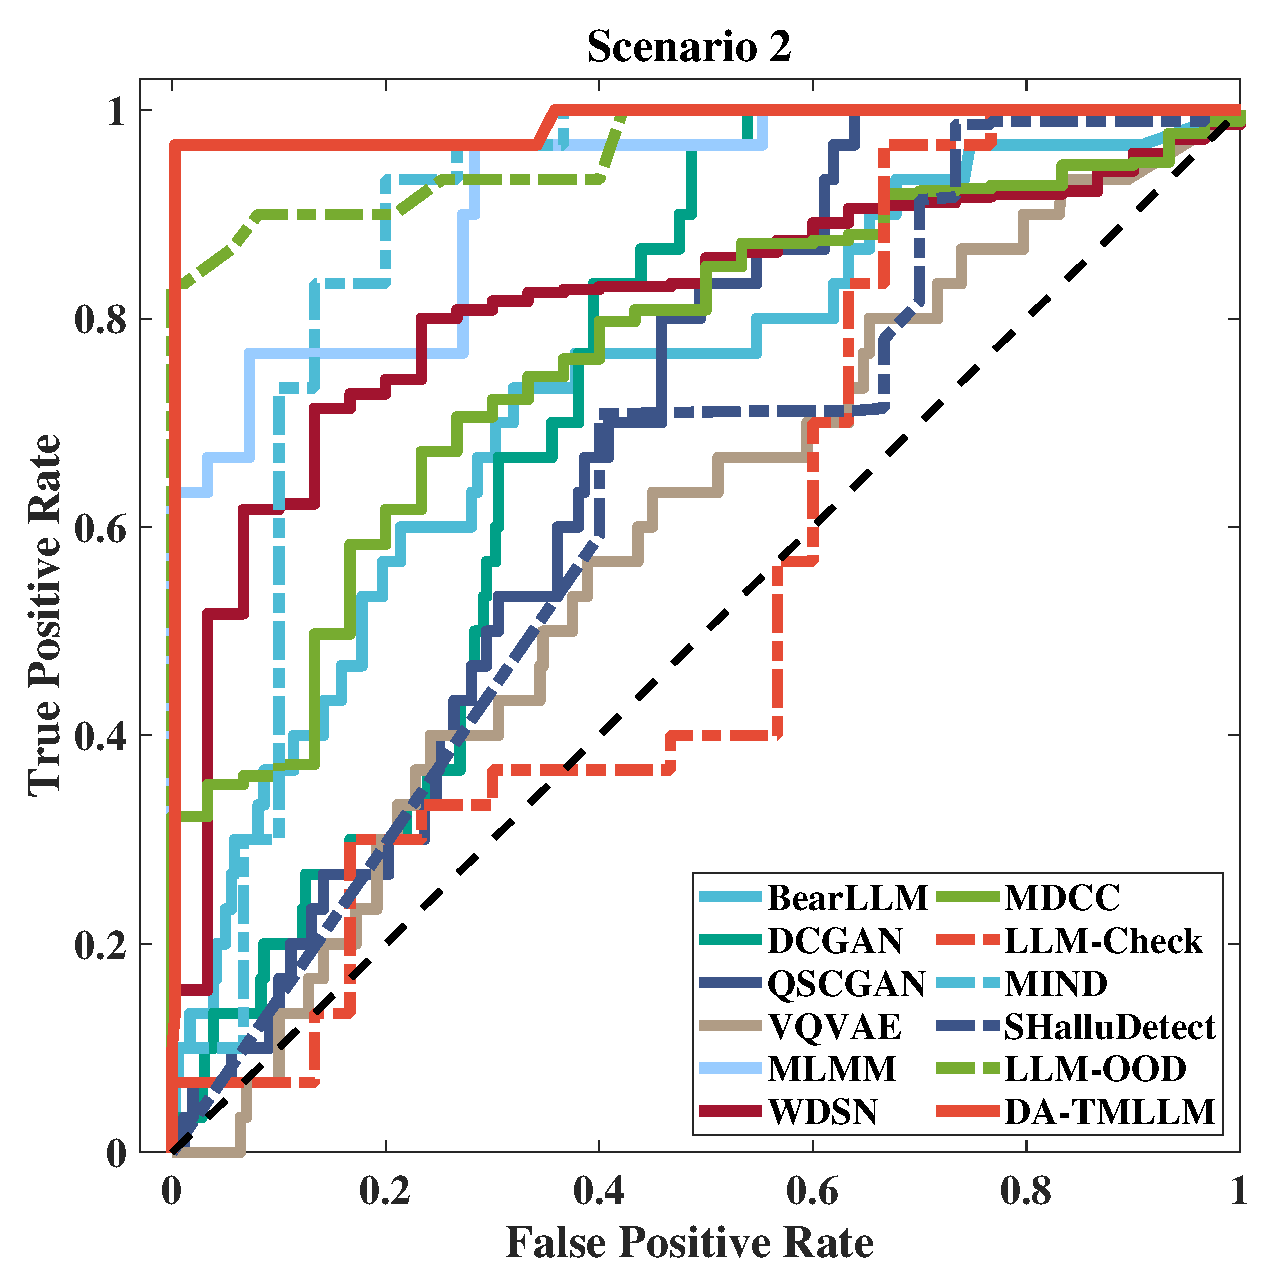
\includegraphics[width=2.3in]{figures/ROC_s2.eps}
		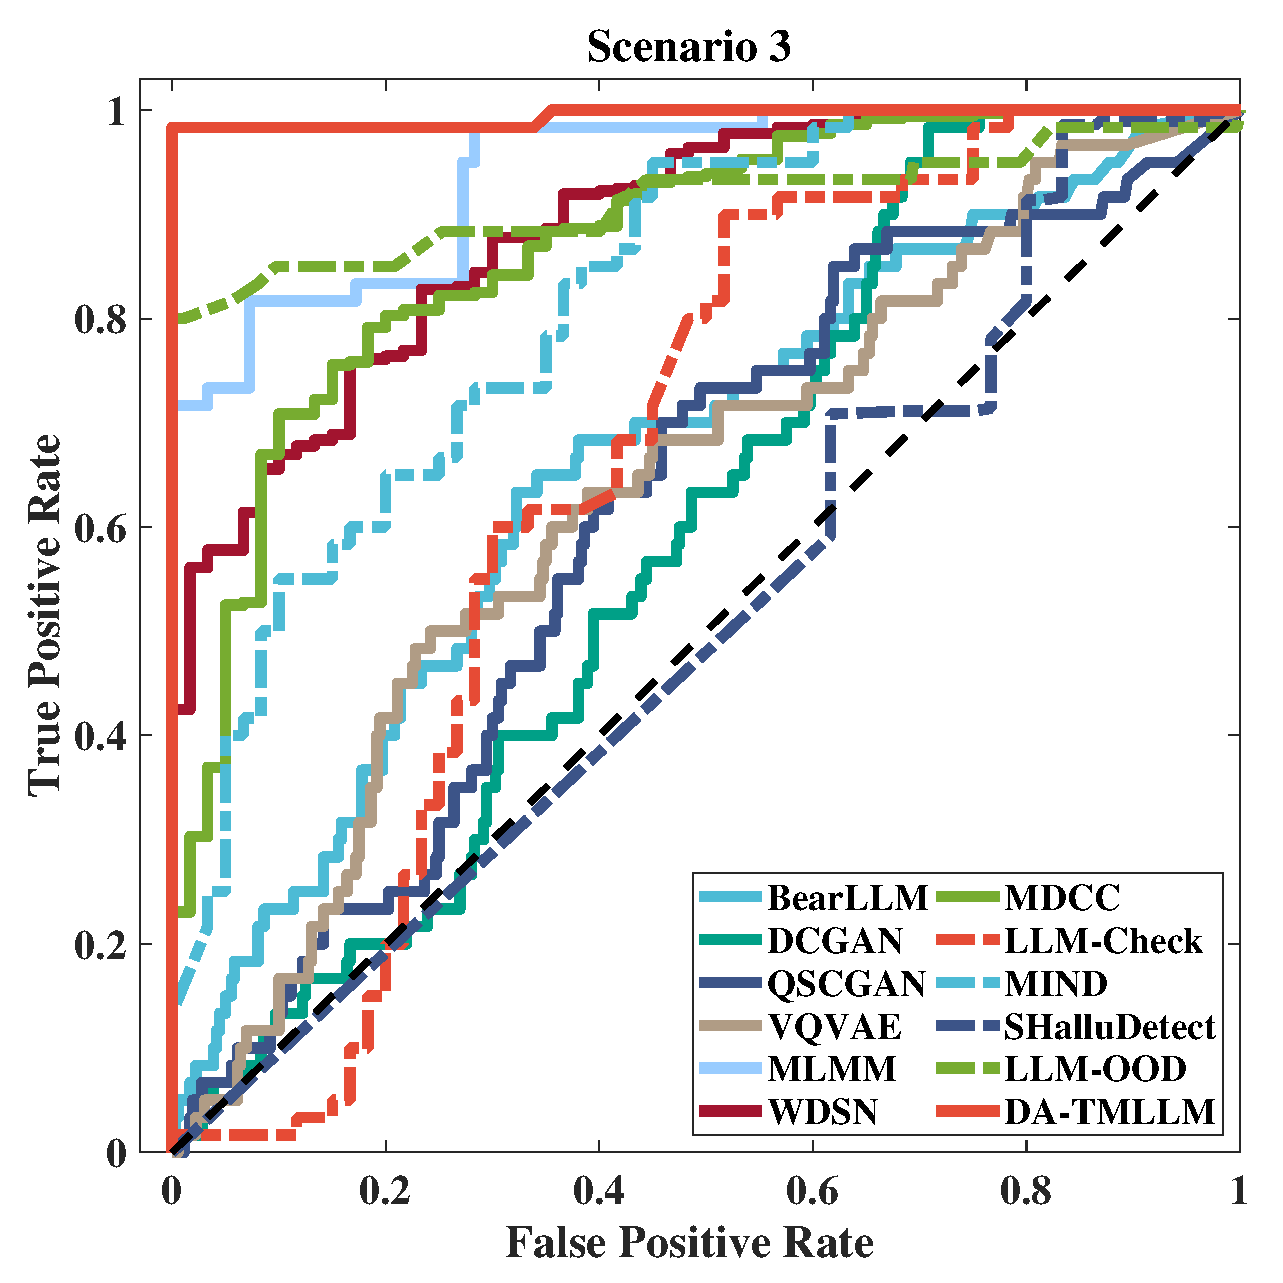
\includegraphics[width=2.3in]{figures/ROC_s3.eps}
	}
	\hfil
	\subfloat[三种场景下的PR曲线]{
		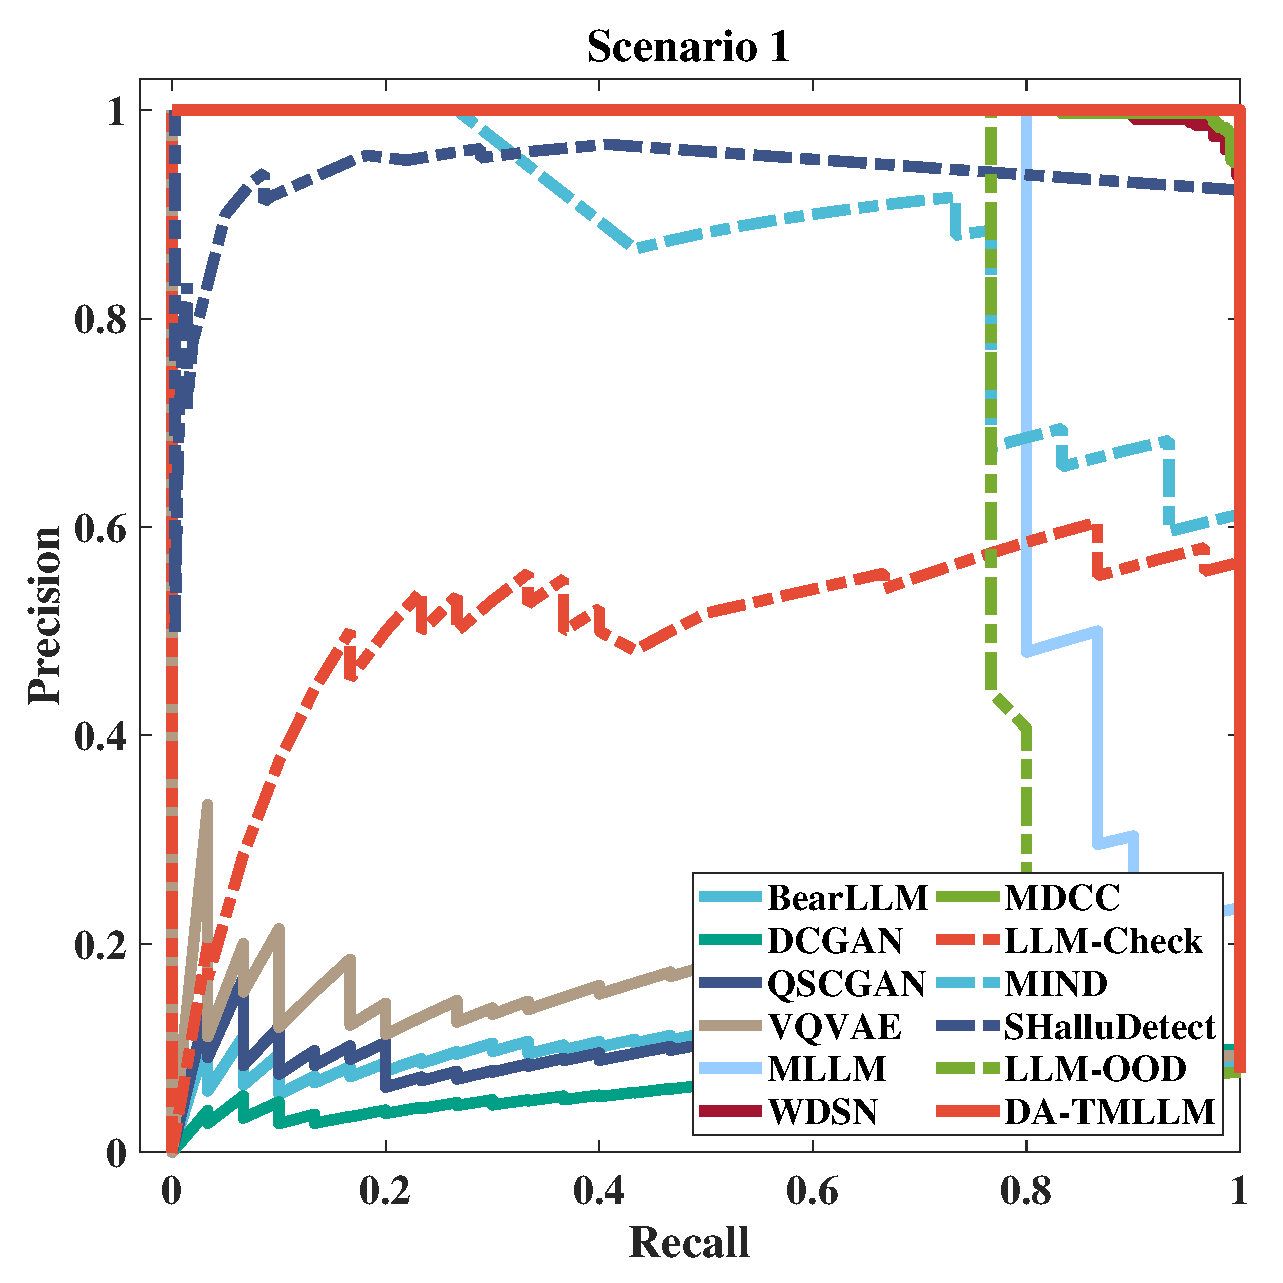
\includegraphics[width=2.3in]{figures/PR_s1.eps}
		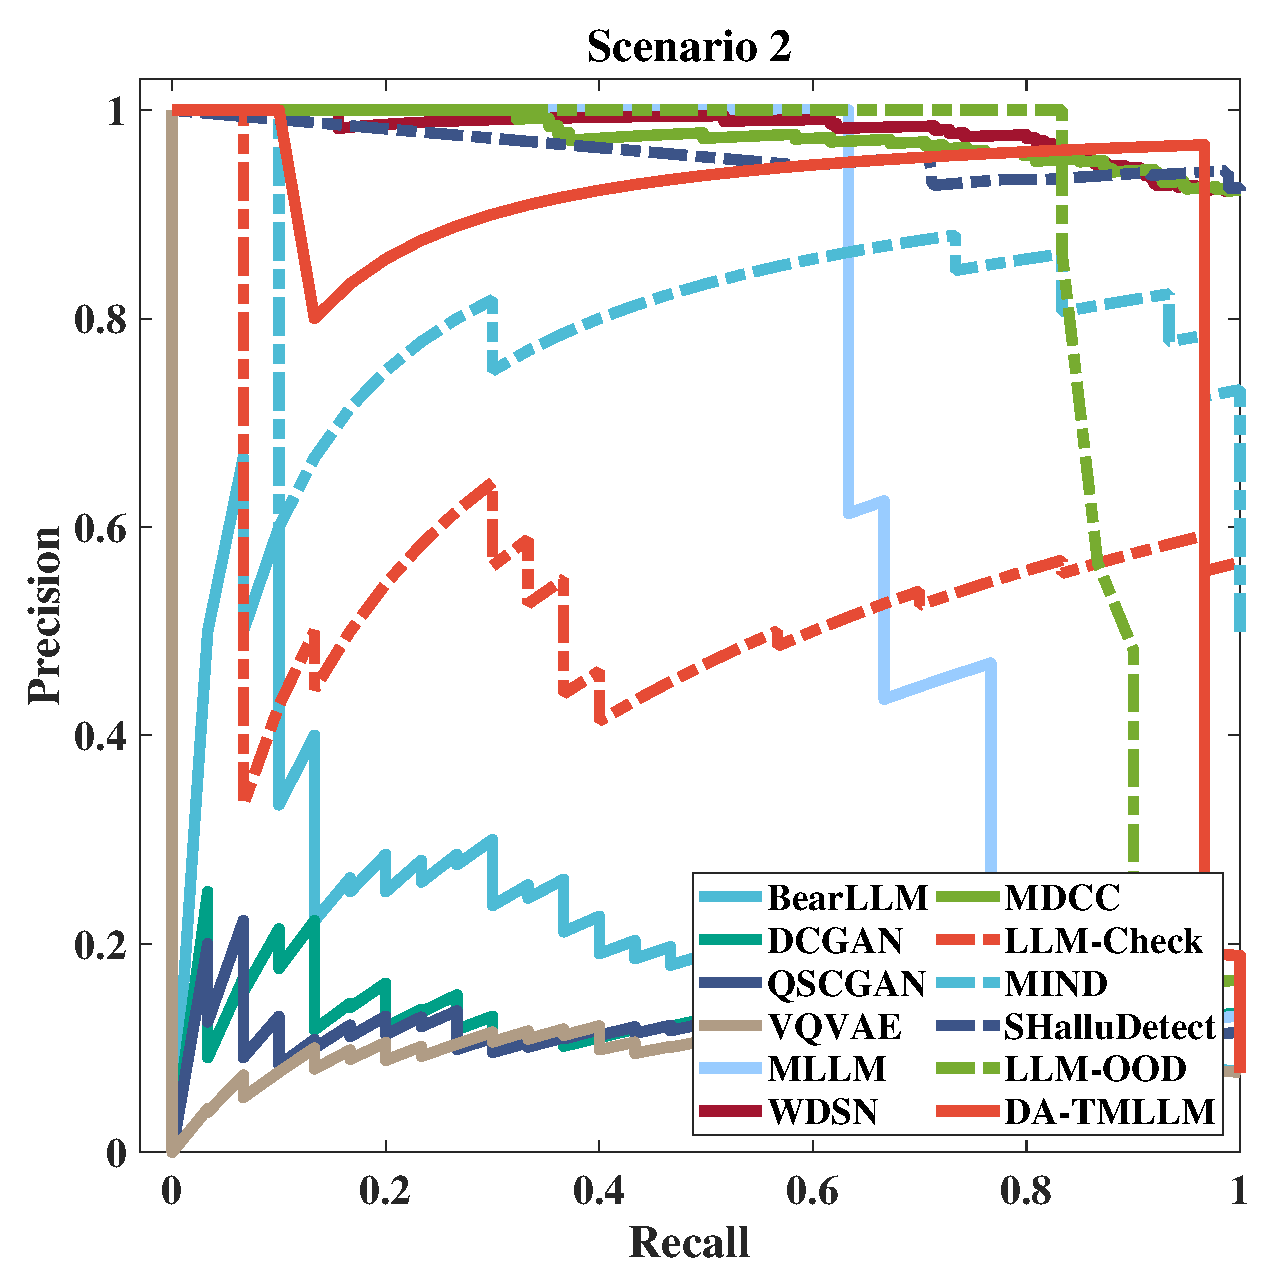
\includegraphics[width=2.3in]{figures/PR_s2.eps}
		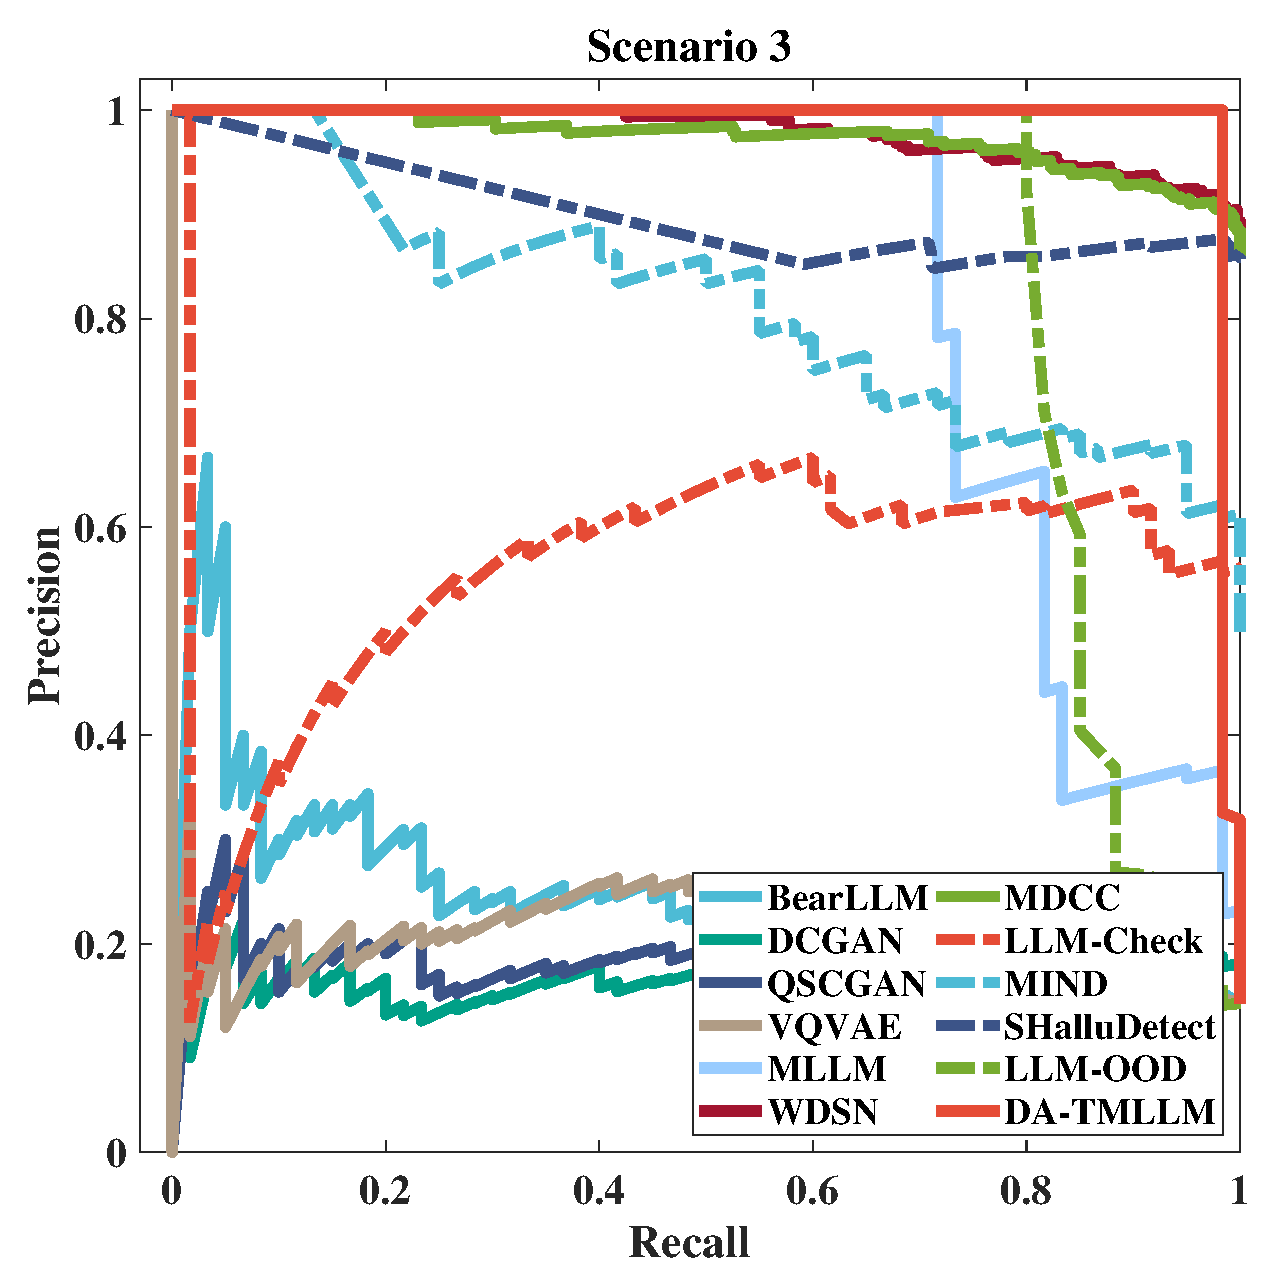
\includegraphics[width=2.3in]{figures/PR_s3.eps}
	}
	\hfil
	% \caption{ROC and PR curves comparing the proposed DA-TMLLM with baseline models for hallucination-resilient diagnosis across the three scenarios.}
	\caption{所提出的DA-TMLLM与基线模型在三种场景下抗幻觉诊断的ROC和PR曲线对比。}
	\label{fig:Performance_Comparison_2}
\end{figure*}

如图\ref{fig:Performance_Comparison_3}所示，我们进一步利用DA-TMLLM和基线模型的扩展混淆矩阵来量化抗幻觉诊断中的两种关键错误类型，即错误接受不期望输入和错误拒绝域特定样本。
扩展混淆矩阵联合呈现了场景3的幻觉检测结果和域特定分类结果。DA-TMLLM的混淆矩阵非常清晰，以对角线为主导，非对角线值最小。它正确拒绝了98\%的不期望输入，且没有拒绝任何域特定样本。然而，基线模型显示出缺陷。BearLLM、DCGAN、QSCGAN和VQVAE遭受大量的错误接受，将不期望输入分散到各种故障类别中。相比之下，具有检测能力的模型(如WDSN和SHalluDetect)表现出高度的错误拒绝，将有效的诊断信号错误分类为不期望输入。该分析直观地证实了DA-TMLLM有效地在准确分布内分类和精确拒绝不期望输入之间进行权衡，从而实现了真正的抗幻觉诊断。
% "As a baseline, we evaluated a model with no specific capability for undesired sample detection. As expected, its FAR@95 score was extremely high, approaching 1. This is because to achieve the 95% recall target, the model's decision threshold must be lowered to a point where it misclassifies nearly all domain-specific samples. This result serves as a sanity check and highlights the challenging nature of the task. In contrast, our proposed model achieves a significantly lower FAR@95 of X.XX, demonstrating its superior ability to distinguish undesired samples with minimal false alarms."

\begin{figure*}[htbp]
	\centering
	% --- 第一行 ---
	\subfloat[BearLLM]{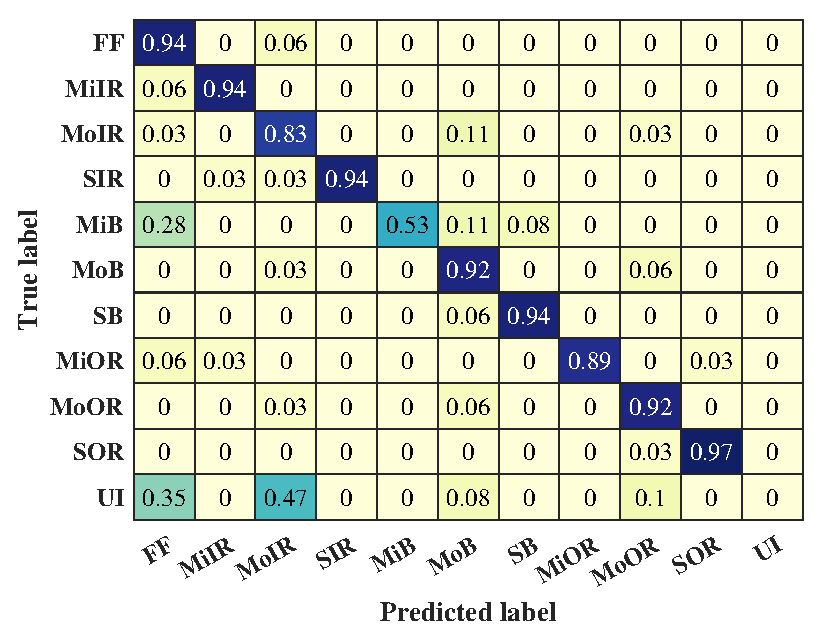
\includegraphics[width=2.3in]{figures/1_BearLLM.eps} \label{fig:sub1}}
	\hfil
	\subfloat[DCGAN]{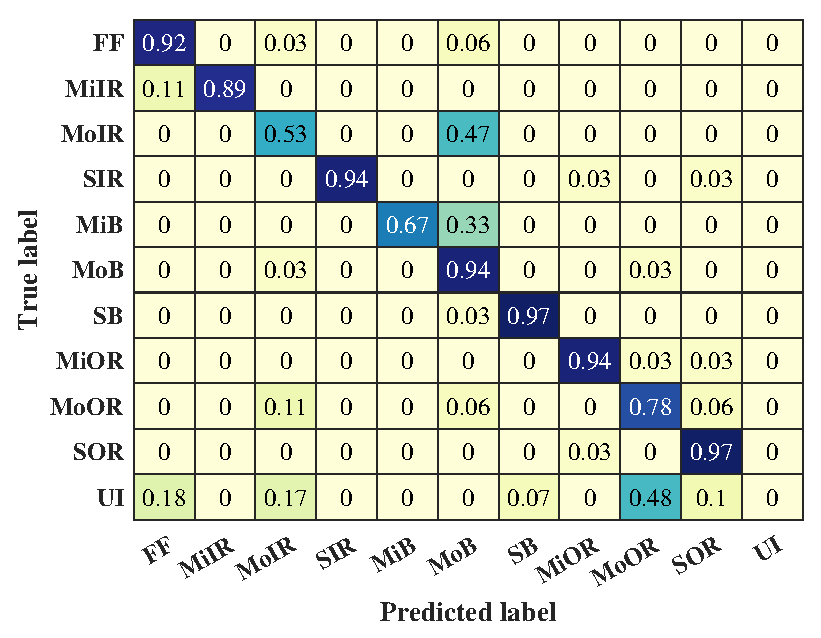
\includegraphics[width=2.3in]{figures/2_DCGAN.eps} \label{fig:sub2}}
	\hfil
	\subfloat[QSCGAN]{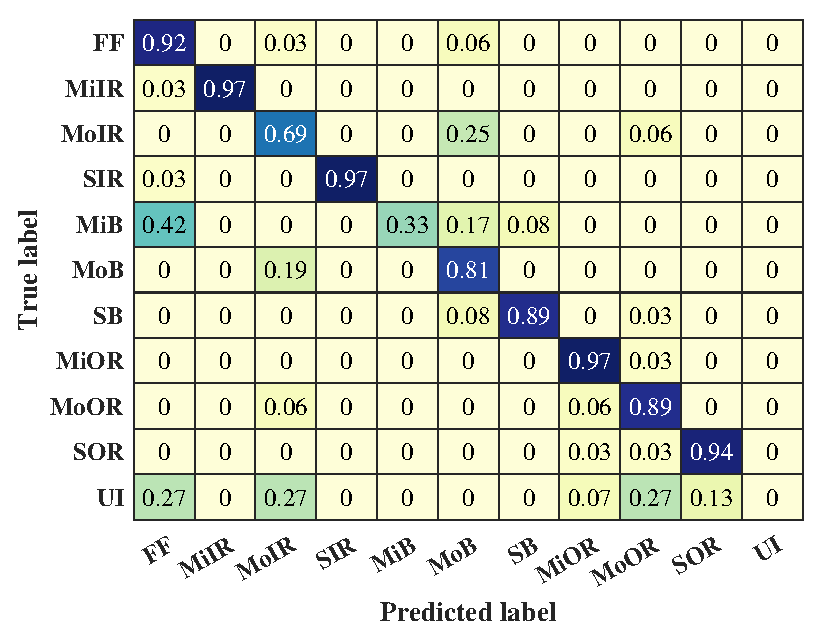
\includegraphics[width=2.3in]{figures/3_QSCGAN.eps} \label{fig:sub3}}
	
	% --- 第二行 ---
	\subfloat[VQVAE]{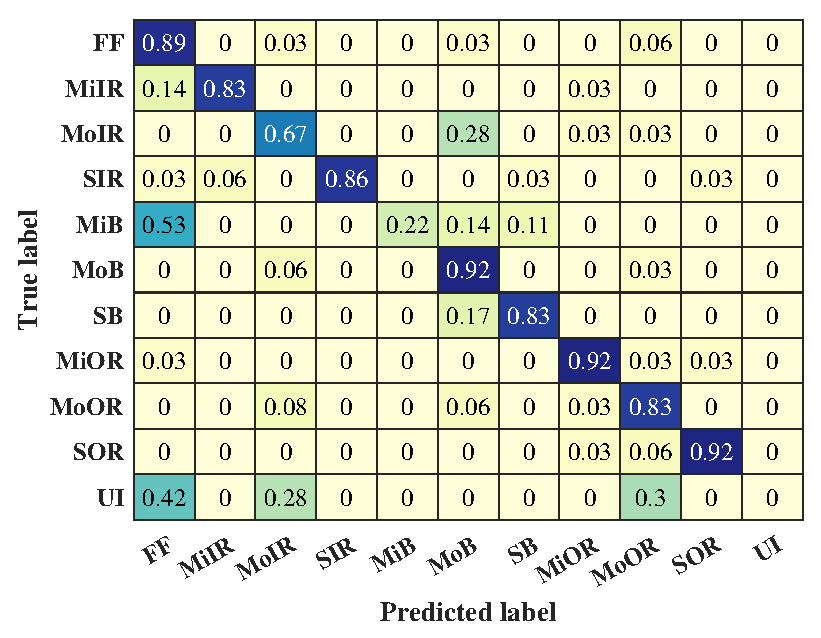
\includegraphics[width=2.3in]{figures/4_VQVAE.eps} \label{fig:sub4}}
	\hfil
	\subfloat[MLMM]{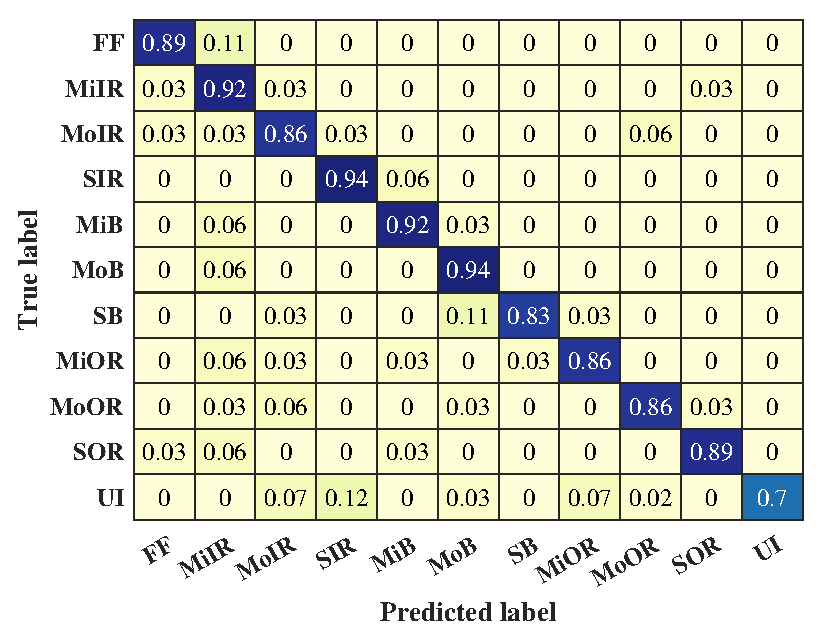
\includegraphics[width=2.3in]{figures/5_MLMM.eps} \label{fig:sub5}}
	\hfil
	\subfloat[WDSN]{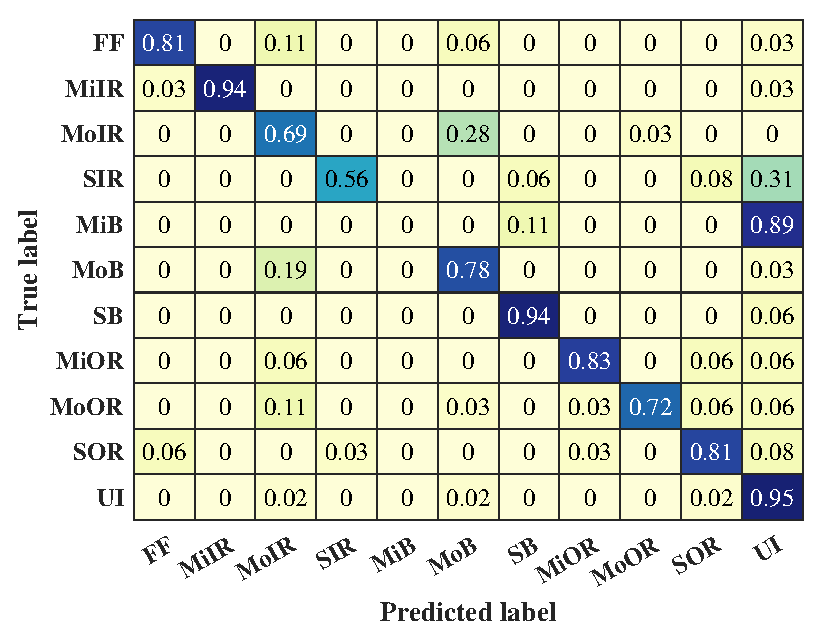
\includegraphics[width=2.3in]{figures/6_WDSN.eps} \label{fig:sub6}}
	
	% --- 第三行 ---
	\subfloat[MDCC]{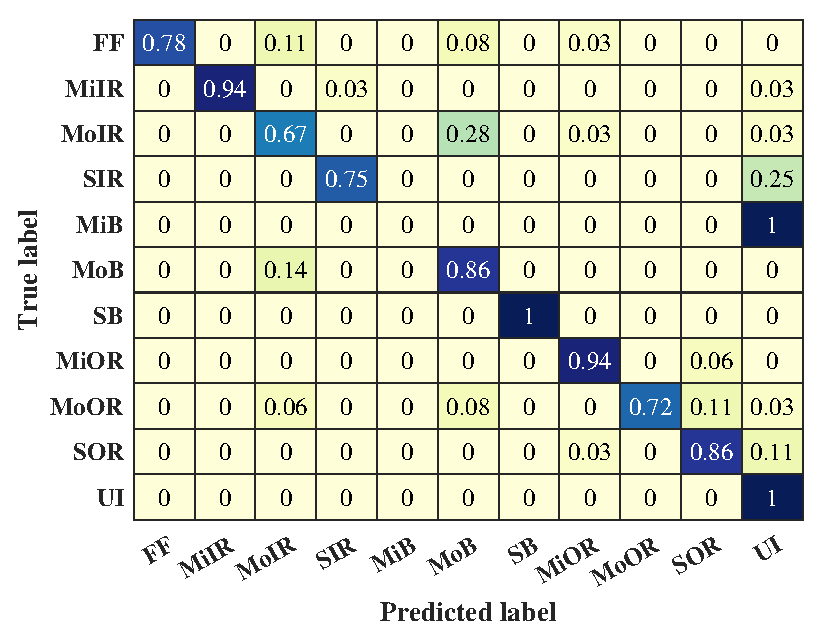
\includegraphics[width=2.3in]{figures/7_MDCC.eps} \label{fig:sub7}}
	\hfil
	\subfloat[LLM-Check]{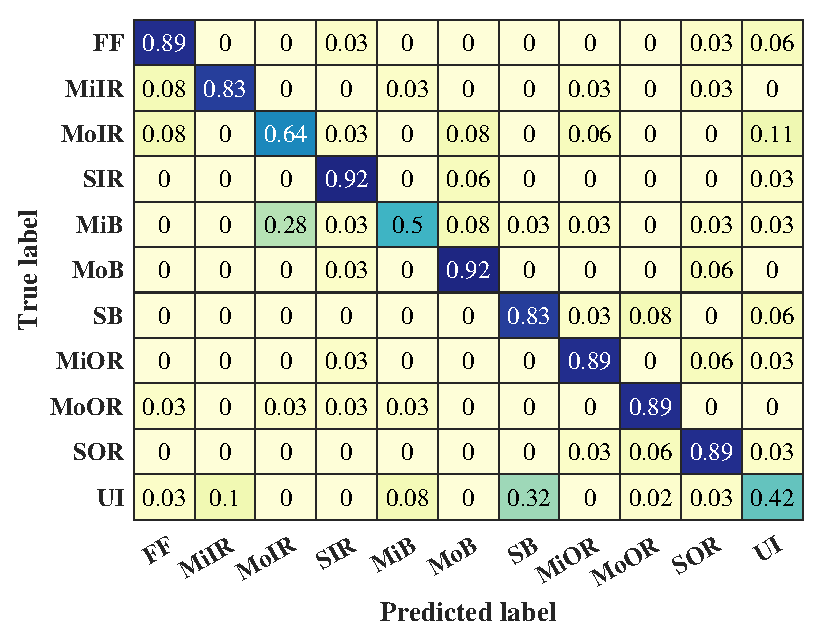
\includegraphics[width=2.3in]{figures/8_LLM-Check.eps} \label{fig:sub8}}
	\hfil
	\subfloat[MIND]{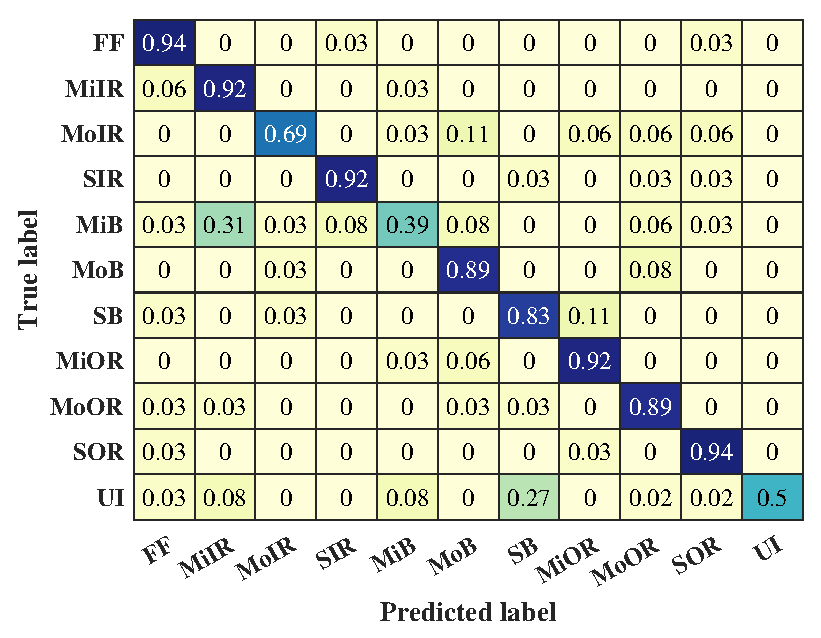
\includegraphics[width=2.3in]{figures/9_MIND.eps} \label{fig:sub9}}
	
	% --- 第四行 ---
	\subfloat[SHalluDetect]{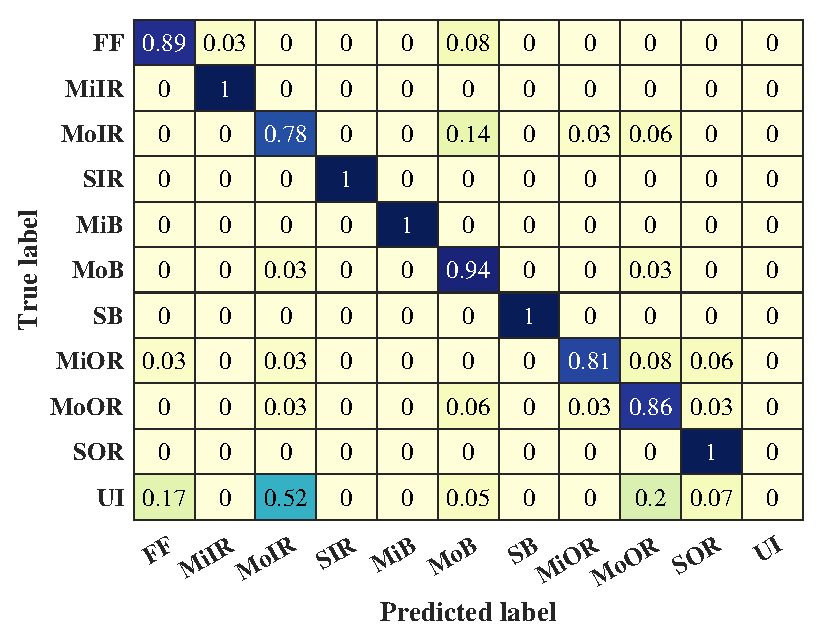
\includegraphics[width=2.3in]{figures/10_SHalluDetect.eps} \label{fig:sub10}}
	\hfil
	\subfloat[LLM-OOD]{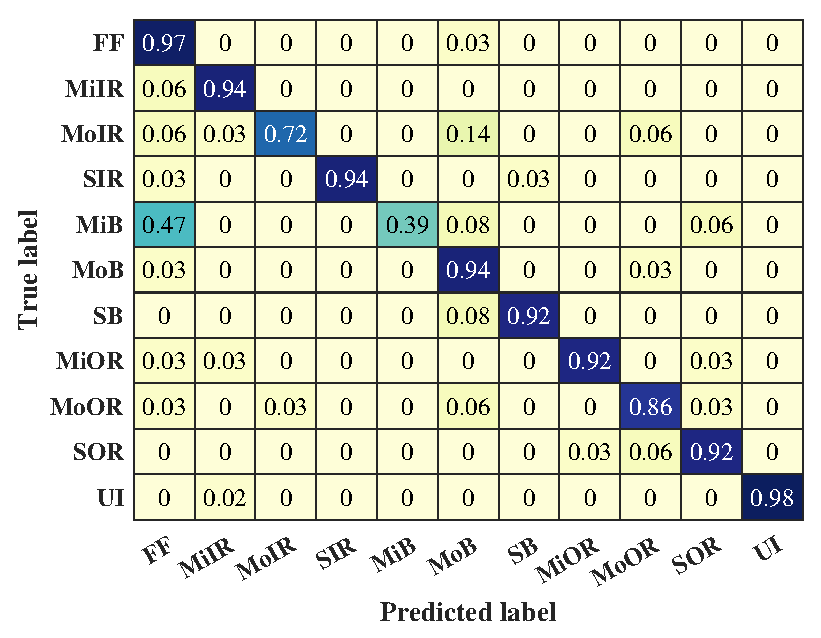
\includegraphics[width=2.3in]{figures/11_LLM-OOD.eps} \label{fig:sub11}}
	\hfil
	\subfloat[DA-TMLLM]{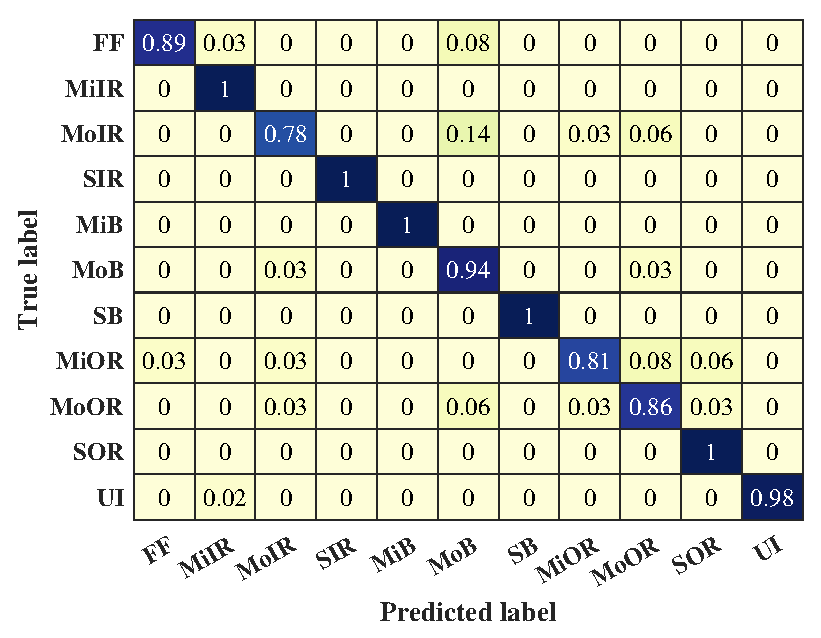
\includegraphics[width=2.3in]{figures/12_DA-TMLLM.eps} \label{fig:sub12}}

	\caption{DA-TMLLM与基线模型在场景3中抗幻觉诊断的扩展混淆矩阵对比。}
	\label{fig:Performance_Comparison_3}
\end{figure*}

我们将DA-TMLLM生成的合成振动信号质量与三个基于增强的基线(包括VQVAE、DCGAN和QSCGAN)在域特定数据集的少数类上进行比较。如表\ref{tab:comparison_result2}所总结，DA-TMLLM实现了最低的RMSE和最高的PSNR与FSCS。定量而言，相对于每种情况下的次佳表现模型，DA-TMLLM平均将RMSE降低了86.9\%，同时将平均PSNR和FSCS提高了97.1\%和67.2\%，验证了其数据增强的优越性。这种优越性能归功于我们的条件扩散模型，它通过引导的渐进去噪过程擅长捕获复杂的非平稳信号特征。相比之下，DCGAN和QSCGAN容易出现训练不稳定性，导致对真实数据分布的捕获不完整，而VQVAE倾向于生成过于平滑、缺乏关键高频细节的信号。

\begin{table*}[t!]
	\footnotesize
	% table caption is above the table
	\caption{基于增强的基线与DE-TMLLM的生成质量对比\textsuperscript{1}}
	\renewcommand{\arraystretch}{1.5}
	\centering
	\label{tab:comparison_result2}       % Give a unique label
	% For LaTeX tables use
	\begin{tabular}{c|c c c|c c c|c c c|c c c}
		\toprule[1pt]\noalign{\vspace{0.5pt}}
		模型&\multicolumn{3}{c|}{VQVAE}&\multicolumn{3}{c|}{DCGAN}&\multicolumn{3}{c|}{QSCGAN}&\multicolumn{3}{c}{DA-TMLLM}
		\\\cmidrule(lr){2-4}\cmidrule(lr){5-7}\cmidrule(lr){8-10}\cmidrule(lr){11-13}
		指标&RMSE &PSNR &FSCS &RMSE &PSNR &FSCS &RMSE &PSNR &FSCS &RMSE &PSNR &FSCS \\\midrule[1pt]
		
		IMS\_MiIR\textsuperscript{2}  & 0.1674 & 15.5231 & 0.0621 & \underline{0.0699} & \underline{23.1205} & \underline{0.4791} & 0.1387 & 17.1660 & 0.4396 & \textbf{0.0084} & \textbf{41.5342} & \textbf{0.9811}
		\\
		\noalign{\vspace{2.8pt}}\hline\noalign{\smallskip}
		IMS\_SB  & 0.4097 & 7.7508 & 0.0460 & \underline{0.1696} & \underline{15.4120} & \underline{0.4823} & 0.2251 & 12.9531 & 0.3099 & \textbf{0.0217} & \textbf{33.3997} & \textbf{0.7835}
		\\
		\noalign{\vspace{2.8pt}}\hline\noalign{\smallskip}
		IMS\_SOR  & 0.7853 & 2.0990 & 0.0239 & \underline{0.1258} & \underline{18.1025} & \underline{0.5693} & 0.1892 & 14.4668 & 0.4196 & \textbf{0.0111} & \textbf{39.1883} & \textbf{0.7418} 
		\\
		\noalign{\vspace{2.8pt}}\hline\noalign{\smallskip}
		PU\_MiIR   & 0.2666 & 11.4819 & 0.0355 & \underline{0.0598} & \underline{24.4715} & \underline{0.4209} & 0.1682 & 15.4824 & 0.2256 & \textbf{0.0108} & \textbf{39.3536} & \textbf{0.7332}
		\\
		\noalign{\vspace{2.8pt}}\hline\noalign{\smallskip}
		XJTU\_MiIR & 0.1269 & 17.9312 & 0.0408 & \underline{0.1177} & \underline{18.6033} & \underline{0.6004} & 0.1902 & 14.4202 & 0.4533 & \textbf{0.0158} & \textbf{36.1506} & \textbf{0.6809}
		\\
		\noalign{\vspace{2.8pt}}\hline\noalign{\smallskip}
		XJTU\_SIR & \underline{0.0464} & \underline{26.6663} & 0.0912 & 0.1665 & 15.7207 & \underline{0.3842} & 0.2041 & 13.8345 & 0.3467 & \textbf{0.0117} & \textbf{38.9643} & \textbf{0.5786}
		\\
		\noalign{\vspace{2.8pt}}\hline\noalign{\smallskip}
		XJTU\_MiB & 0.1729 & 15.2460 & 0.0865 & 0.1685 & 15.4795 & 0.5216 & \underline{0.1541} & \underline{16.2510} & \underline{0.5346} & \textbf{0.0163} & \textbf{35.8361} & \textbf{0.7601} 
		\\
		\noalign{\vspace{2.8pt}}\hline\noalign{\smallskip}
		XJTU\_SB & 0.4908 & 6.1818 & 0.0256 & \underline{0.1007} & \underline{20.0536} & \underline{0.4464} & 0.2295 & 12.8102 & 0.3242 & \textbf{0.0099} & \textbf{40.0970} & \textbf{0.7360}
		\\
		\noalign{\vspace{2.8pt}}\hline\noalign{\smallskip}
		XJTU\_SOR & 0.3577 & 8.9290 & 0.0407 & \underline{0.1464} & \underline{16.6960} & \underline{0.2624} & 0.1865 & 14.5998 & 0.3848 & \textbf{0.0102} & \textbf{39.9638} & \textbf{0.6873}
		\\
		%		
		\noalign{\vspace{0.5pt}}
		\bottomrule[1pt]
		\multicolumn{13}{l}{\textsuperscript{1} 最佳结果：\textbf{粗体}；次佳结果：\underline{下划线}。}\\[-5pt]
		\multicolumn{13}{l}{\textsuperscript{2} IMS\_MiIR表示对IMS数据集中的MiIR类别应用数据增强。}\\[-5pt]
	\end{tabular}
\end{table*}

\subsection{消融研究}
我们进行消融研究以量化DA-TMLLM每个主要组件的贡献。
如表\ref{tab:ablation_study}所示，报告了三个场景中消融研究的实验结果，包括DS-ACC、G-ACC、AUROC、FAR@95和AUPR。

\subsubsection{去除ControlNet} 我们将ControlNet模块替换为大核深度卷积神经网络，从而移除条件引导，将模型恢复为传统的去噪扩散概率模型。该变体在所有三个场景中都表现出性能下降，表明ControlNet对于从各种故障类型和工况的振动信号中提取判别特征至关重要。

\subsubsection{去除CGCDM} 我们移除所提出的ControlNet引导跨数据集条件扩散模块，仅使用原始的、不平衡的故障信号训练诊断模型。这导致诊断准确率下降。这一发现突显了我们基于扩散的故障模式增强的有效性，强调了其在缓解统计偏差和纠正数据不平衡造成的扭曲决策边界方面的作用。

\subsubsection{去除KTURS} 我们将所提出的token级不确定性(如式\eqref{equa:token_level_uncertainty}所定义)替换为式\eqref{equa:normalized_energy_score}中的归一化能量分数。我们观察到不期望输入识别性能下降，如AUROC、FAR@95和AUPR所衡量。这一结果证明了设计的关键token不确定性重加权策略对检测序列级幻觉的有效性。

\subsubsection{去除TMLLM} 我们移除可信多模态大语言模块，从而消除了框架的幻觉检测能力，导致不期望输入识别性能下降。这一结果证实了所提出的方法能够有效量化不确定性并提供可信的诊断回答。

\setlength{\tabcolsep}{1pt}
\begin{table*}[t!]
	\footnotesize
	% table caption is above the table
	\caption{三种场景下消融研究的实验结果\textsuperscript{1}}
	\renewcommand{\arraystretch}{1.5}
	\centering
	\label{tab:ablation_study}       % Give a unique label
	% For LaTeX tables use
	\begin{tabular}{c|ccccc|ccccc|ccccc}
		\toprule[1pt]\noalign{\vspace{0.5pt}}
		场景&\multicolumn{5}{c|}{场景1}&\multicolumn{5}{c|}{场景2}&\multicolumn{5}{c}{场景3}
		\\\cmidrule(lr){2-6}\cmidrule(lr){7-11}\cmidrule(lr){12-16}
		指标&DS-ACC &G-ACC &AUROC &FAR@95 &AUPR &DS-ACC &G-ACC &AUROC &FAR@95 &AUPR &DS-ACC &G-ACC &AUROC &FAR@95 &AUPR \\\midrule[1pt] 
		去除ControlNet\textsuperscript{2}
		& \underline{89.17\%} & 89.74\% & \textbf{1.0000} & \textbf{0.0000} & \textbf{1.0000} & \underline{89.17\%} & 89.74\% & \textbf{1.0000} & \textbf{0.0000} & \textbf{1.0000} & \underline{89.17\%} & 90.48\% & \textbf{1.0000} & \textbf{0.0000} & \textbf{1.0000} \\
		\noalign{\vspace{2.8pt}}\hline\noalign{\smallskip}
		去除CGCDM\textsuperscript{4}
		& 87.50\% & 88.21\% & \textbf{1.0000} & \textbf{0.0000} & \textbf{1.0000} & 87.50\% & 88.21\% & \textbf{1.0000} & \textbf{0.0000} & \textbf{1.0000} & 87.50\% & 89.05\% & \textbf{1.0000} & \textbf{0.0000} & \textbf{1.0000} \\
		\noalign{\vspace{2.8pt}}\hline\noalign{\smallskip}
		去除KTURS\textsuperscript{3}
		& \textbf{92.78\%} & \underline{92.05\%} & \underline{0.9284} & \underline{0.5222} & \underline{0.6579} & \textbf{92.78\%} & \underline{91.54\%} & 0.9251 & 0.2861 & 0.7205 & \textbf{92.78\%} & \underline{91.19\%} & 0.9268 & \underline{0.2861} & 0.7773 \\
		\noalign{\vspace{2.8pt}}\hline\noalign{\smallskip}
		去除TMLLM\textsuperscript{5}
		& \textbf{92.78\%} & 85.64\% & 0.7073 & 1.0000 & 0.1895 & \textbf{92.78\%} & 85.64\% & 0.8625 & 0.6306 & 0.3898 & \textbf{92.78\%} & 79.52\% & 0.7851 & 1.0000 & 0.4210 \\
		\noalign{\vspace{2.8pt}}\hline\noalign{\smallskip}
		DA-TMLLM
		& \textbf{92.78\%} & \textbf{93.33\%} & \textbf{1.0000} & \textbf{0.0000} & \textbf{1.0000} & \textbf{92.78\%} & \textbf{92.82\%} & \underline{0.9860} & \underline{0.0028} & \underline{0.9092} & \textbf{92.78\%} & \textbf{93.57\%} & \underline{0.9942} & \textbf{0.0000} & \underline{0.9887} \\
		%		
		\noalign{\vspace{0.5pt}}
		\bottomrule[1pt]
		\multicolumn{13}{l}{\textsuperscript{1} 最佳结果：\textbf{粗体}；次佳结果：\underline{下划线}。}\\	[-5pt]
		\multicolumn{13}{l}{\textsuperscript{2} 去除ControlNet表示在消融研究中移除ControlNet。}\\	[-5pt]
		\multicolumn{13}{l}{\textsuperscript{3} 去除KTURS表示在消融研究中移除KTURS。}\\	[-5pt]
		\multicolumn{16}{l}{\textsuperscript{4} 去除CGCDM表示在消融研究中移除抗幻觉方案中的CGCDM。}\\	[-5pt]
		\multicolumn{16}{l}{\textsuperscript{5} 去除TMLLM表示在消融研究中移除抗幻觉方案中的TMLLM。}\\	[-5pt]
	\end{tabular}
\end{table*}
\setlength{\tabcolsep}{6pt}

\begin{figure*}[htbp]
	\centering
	\subfloat{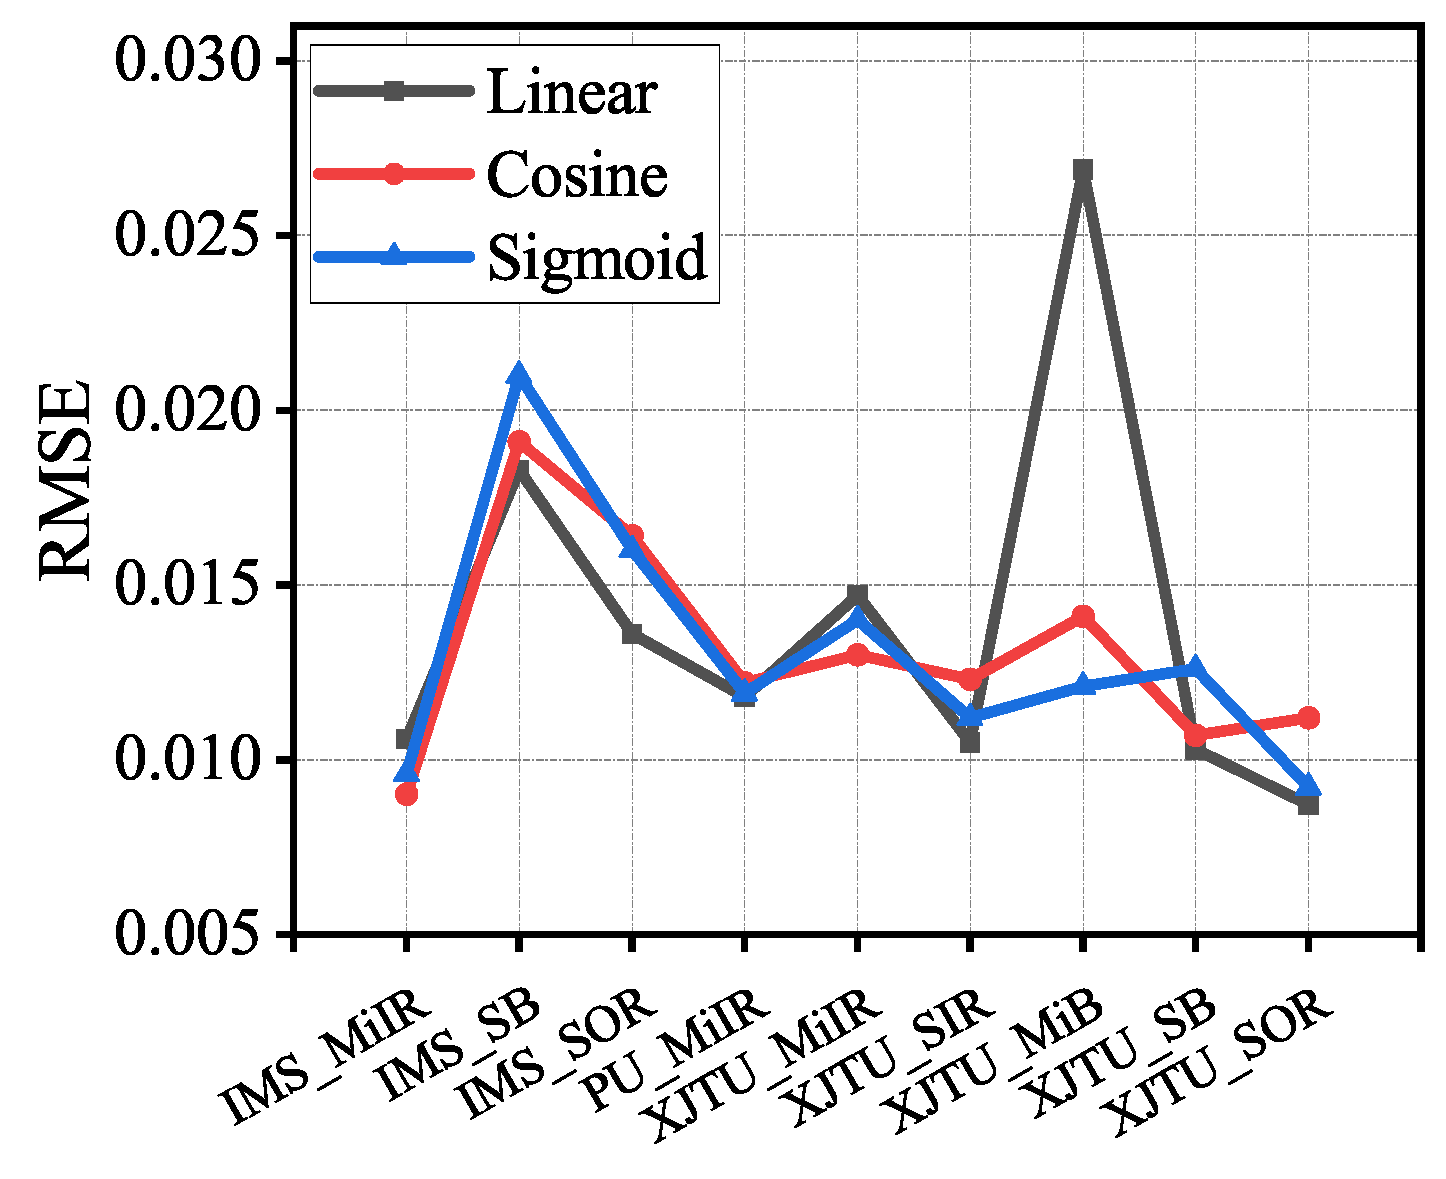
\includegraphics[width=1.75in]{figures/sa1.eps} \label{fig:sa1}}
	\subfloat{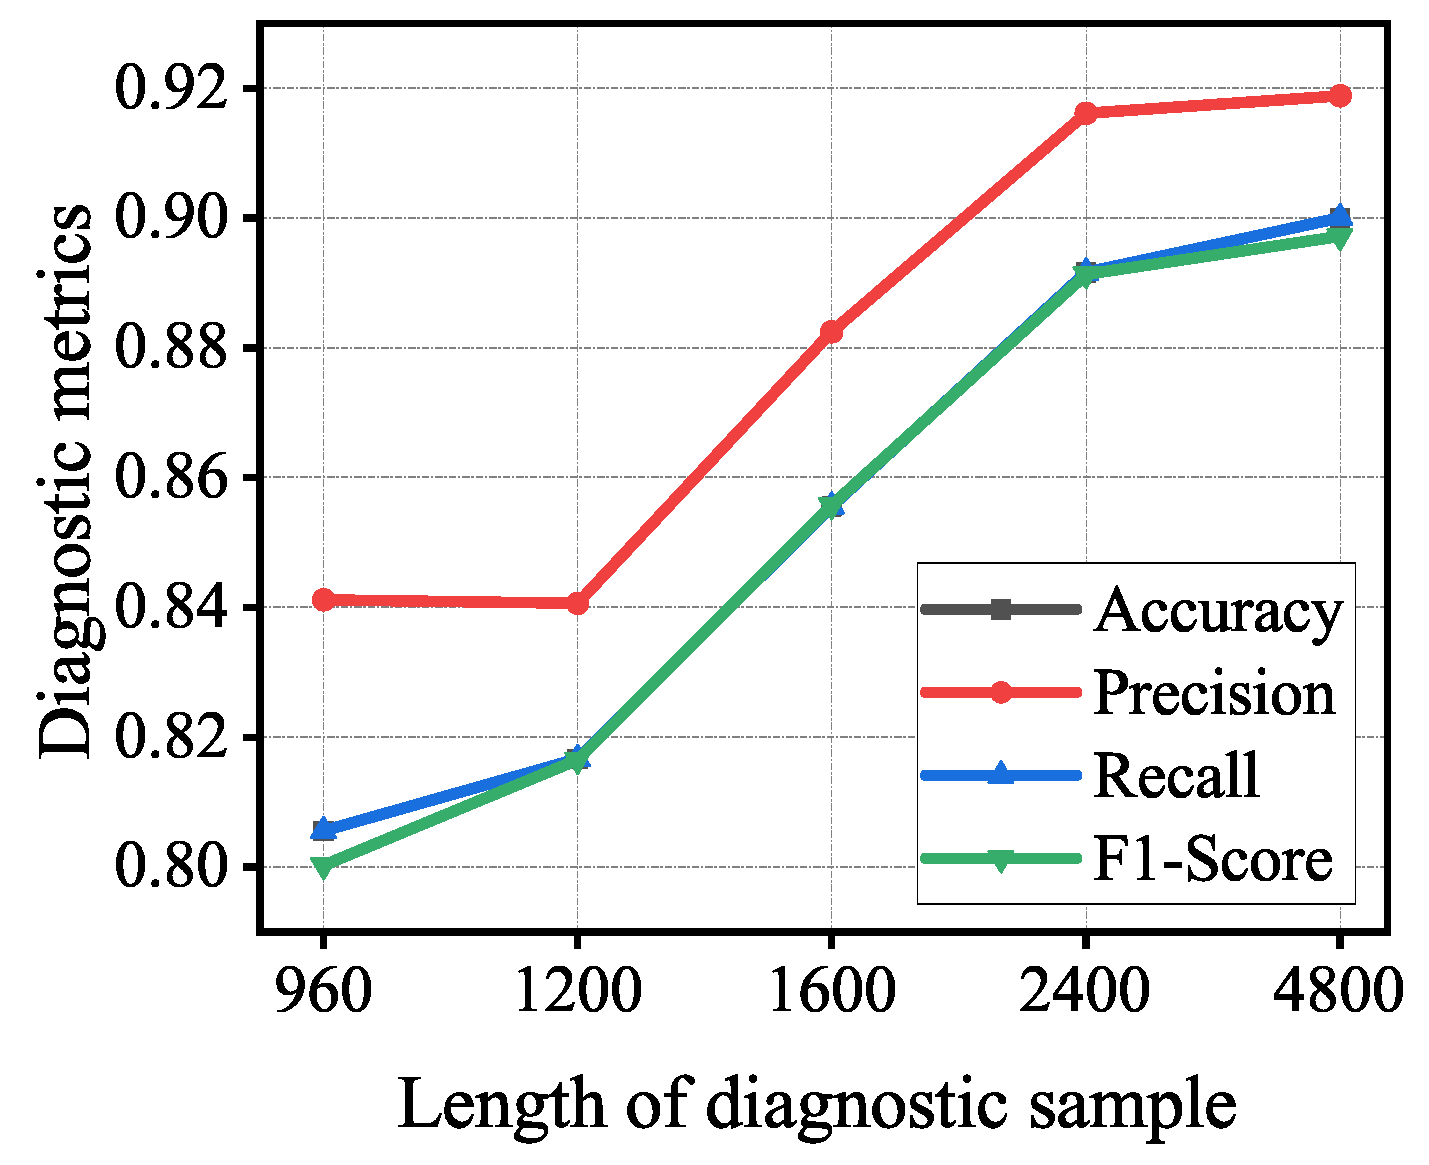
\includegraphics[width=1.75in]{figures/sa2.eps} \label{fig:sa2}}
	\subfloat{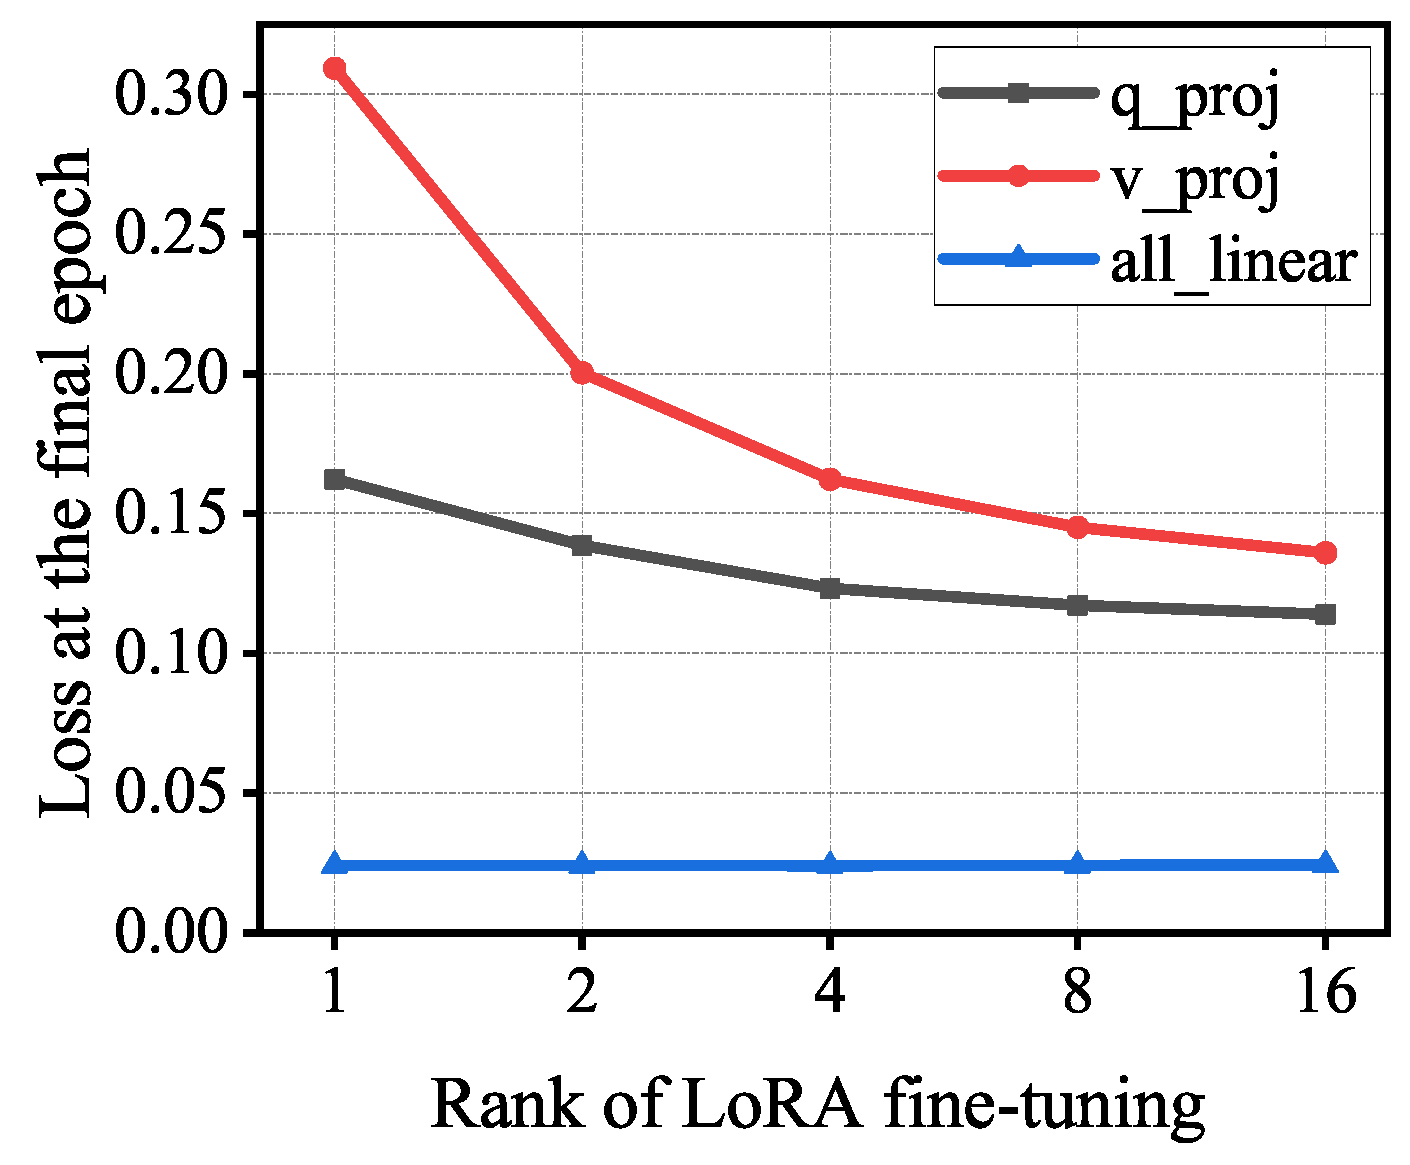
\includegraphics[width=1.75in]{figures/sa3.eps} \label{fig:sa3}}
	\subfloat{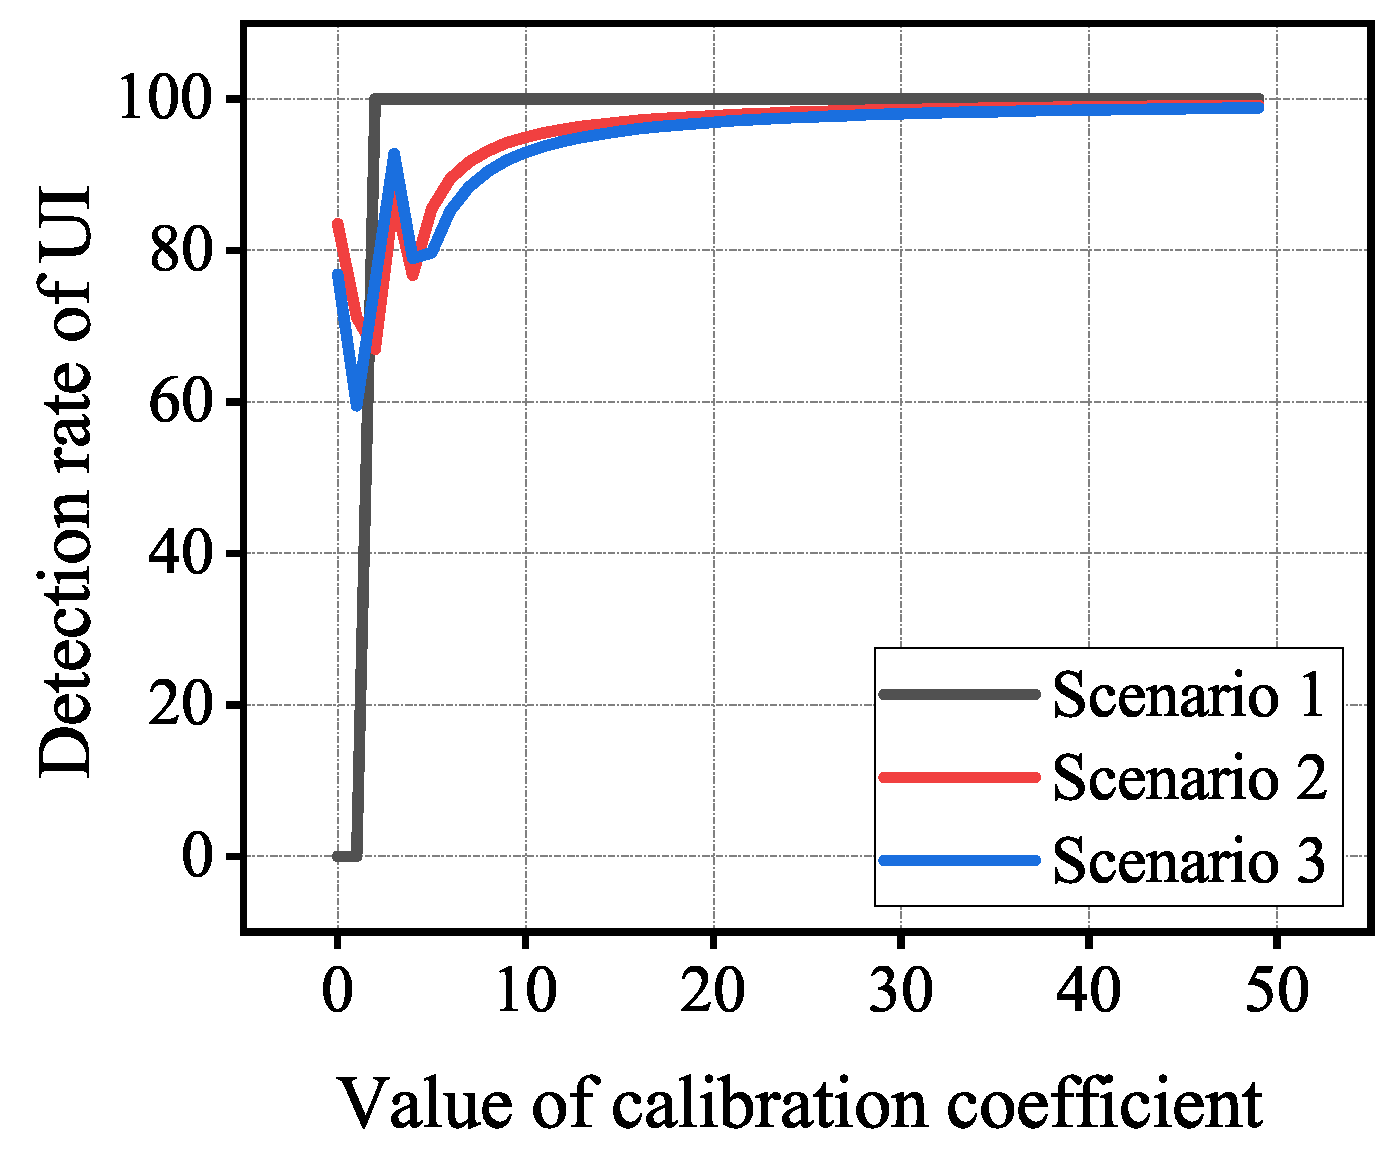
\includegraphics[width=1.75in]{figures/sa4.eps} \label{fig:sa4}}
	
	\caption{DA-TMLLM性能对扩散噪声调度器、诊断信号长度、LoRA微调秩和校准系数的超参数敏感性分析。}
	\label{fig:Sensitivity_Analysis}
\end{figure*}

\subsection{超参数敏感性分析}

为评估DA-TMLLM性能对其超参数的敏感性，我们在MBHM、MaFaulDa和UP数据集上进行了分析。该实验研究了扩散模型的噪声调度器$\zeta$、诊断信号长度$L_{f}$、LoRA微调秩$r_{LoRA}$和关键token校准系数$\omega$的影响。这些参数的影响分别通过生成信号与真实信号之间的RMSE、ControlNet在已知类别上的诊断准确率、最终微调轮次的二元交叉熵损失和不期望输入的检测率来评估。

\subsubsection{$\zeta$的影响} 我们评估了线性、余弦和Sigmoid噪声调度器，发现线性方法在大多数故障类型上产生了更优的信号重建，如图\ref{fig:Sensitivity_Analysis}所示。其均匀的噪声添加更好地与故障信号重建的归纳偏差对齐，而非线性调度器可能损害生成稳定性。

\subsubsection{$L_{f}$的影响} 我们通过测试$\{960, 1200, 1600, 2400, 4800\}$中的值来研究诊断信号长度对DA-TMLLM性能的影响。如图\ref{fig:Sensitivity_Analysis}所示，诊断准确率随信号长度增加而提高。较短的信号缺乏足够的判别信息，而过长的信号可能在扩散过程中造成GPU内存瓶颈。因此，我们选择
$L_{f} = 2400$以平衡诊断效能和计算开销。

\subsubsection{$r_{LoRA}$的影响} 由于LoRA设置会影响微调期间的文本-信号对对齐，我们针对值投影($v\_proj$)、查询投影($q\_proj$)和所有线性层($all\_linear$)进行了实验。这些模块的可训练参数分别占模型总数的0.0130\%、0.0223\%和0.300\%。我们从$\{1, 2, 4, 8, 16\}$中选择LoRA秩$r_{LoRA}$。如图\ref{fig:Sensitivity_Analysis}所示，文本-信号对齐性能随可训练参数数量和LoRA秩的增加而提高。当针对所有线性层且$r_{LoRA} = 4$时，达到了最低损失$0.0240$，与表\ref{tab:Hyperparameter}中的最优参数一致。

\subsubsection{$\omega$的影响} 我们在范围$\{1, 2, \cdots, 50\}$内评估不确定性校准系数$\omega$对不期望输入检测的影响。如图\ref{fig:Sensitivity_Analysis}所示，较大的系数增强了DA-TMLLM检测不期望token的能力。这是因为它更准确地量化了无偏token级不确定性，从而放大了域特定token和不期望token之间的分布差异。

\section{结论}
在本文中，我们提出了DA-TMLLM，一种检测和缓解诊断LLM幻觉的新方法。
首先，我们设计了一个ControlNet引导的跨数据集条件扩散模型，通过注入可控语义引导和合成多样化样本来缓解统计偏差。
其次，我们设计了TMLLM，通过点二列相关分析和显著性检验来定位关键token，并设计关键token驱动的不确定性重加权策略，以增强幻觉检测性能。
第三，我们设计了一个抗幻觉方案，将基于扩散的增强和TMLLM整合到一个统一的流程中，用于幻觉检测和缓解。
在十一个故障诊断数据集上获得的评估结果表明，DA-TMLLM在八个指标上始终优于十一个对比模型。

\bibliographystyle{IEEEtran}
\bibliography{refs}
\newpage
\vfill

\end{document}
